\documentclass[../notes.tex]{subfiles}

\pagestyle{main}
\renewcommand{\chaptermark}[1]{\markboth{\chaptername\ \thechapter\ (#1)}{}}
\stepcounter{chapter}

\begin{document}




\chapter{Interpreting Spectra}
\section{Lecture 3: Time, Frequency, and Fourier Transforms}
\begin{itemize}
    \item \marginnote{1/10:}Frequency- and time-domain spectroscopy.
    \begin{itemize}
        \item Two ways of extracting the same information.
        \begin{enumerate}
            \item Absorption spectrum (frequency domain).
            \begin{itemize}
                \item Vary frequency of driving field or disperse white light after passing through the sample and look at each frequency component.
                \item Measure the power absorbed for different frequencies.
                \item Tells us the resonance frequency, how strongly the light interacts with the matter, and damping times or relaxation processes.
            \end{itemize}
            \item Pulsed excitation (time domain).
            \begin{itemize}
                \item Apply a pulsed driving force.
                \item Measure resultant periodic oscillation and relaxation.
                \item This is the basis for modern NMR and FTIR instruments.
            \end{itemize}
        \end{enumerate}
        \item Both represent the time-dependent behavior of a molecule.
    \end{itemize}
    \item A powerful reason to use the time domain is the formal relationship between time and frequency data, the \textbf{Fourier transform}.
    \item \textbf{Fourier transform}: A formal relationship between the time domain and the frequency domain.
    \begin{itemize}
        \item Underlying idea: Any function can be expressed as a sum of sines and cosines, i.e.,
        \begin{equation*}
            F(t) = \sum_{n=1}^\infty[a_n\cos(n\bar{\omega}t)+b_n\sin(n\bar{\omega}t)]
        \end{equation*}
        \item In practice, sample $N$ points over a period $T$.
        \begin{itemize}
            \item The values of time at which we sample are $t=n\delta t$ for $n=1,\dots,m$.
        \end{itemize}
        \item Numerical analysis: Expand in harmonics of base frequency, i.e., we let $\bar{\omega}=\pi/T$ be 1/2 cycle of $T$. The harmonics are $n\bar{\omega}$ for $n=1$ to $N$. We thus have as many harmonics as we do data points.
        \item Then we plot the expansion coefficients vs. the frequency, and that is the spectrum in the series of expansion coefficients.
        \item There's more to it than this, but this is the basic concept.
        \item Also, this is only a discrete data set.
    \end{itemize}
    \item \textbf{Fourier analysis}: Determining the coefficients $a_n,b_n$.
    \item Fourier transform relations.
    \begin{itemize}
        \item For continuous functions, we use Fourier transform integrals.
        \begin{itemize}
            \item Note that although both of the following integrals are sine transforms, there also exist cosine and complex $\e[-i\omega t]$ transforms.
            \item Sine and cosine transforms are used for real data; the complex form is more general.
        \end{itemize}
        \item To convert to the time domain $S(t)$, we write
        \begin{equation*}
            S(t) = \frac{1}{\sqrt{2\pi}}\int_{-\infty}^{+\infty}\tilde{S}(\omega)\sin\omega t\dd\omega
        \end{equation*}
        \item To convert to the frequency domain $\tilde{S}(\omega)$, we write
        \begin{equation*}
            \tilde{S}(\omega) = \frac{1}{\sqrt{2\pi}}\int_{-\infty}^{+\infty}S(t)\sin\omega t\dd{t}
        \end{equation*}
        \item Example: Damped harmonic oscillator.
        \begin{equation*}
            S(t) \propto \e[-\gamma t]\sin\omega_0t
            \quad\Longleftrightarrow\quad
            \tilde{S}(\omega) \propto \frac{\gamma}{(\omega-\omega_0)^2+\gamma^2}
        \end{equation*}
    \end{itemize}
    \item Parameters in the time and frequency domains.
    \begin{figure}[h!]
        \centering
        \begin{tikzpicture}
            \footnotesize
            \begin{scope}
                \draw [-latex] (0,0) -- (5,0) node[below left]{$t$};
                \node at (-1,2.75) {\small$S(t)$};
    
                \draw [blx,yshift=4.7cm,yscale=0.5] plot[domain=0:5,samples=1000,smooth,/pgf/fpu,/pgf/fpu/output format=fixed] (\x,{e^(-0.5*\x)*sin(50*\x r)});
                \draw [grx,yshift=3.4cm,yscale=0.5] plot[domain=0:5,samples=1000,smooth,/pgf/fpu,/pgf/fpu/output format=fixed] (\x,{e^(-1.5*\x)*sin(50*\x r)});
                \draw [orx,yshift=2.1cm,yscale=0.5] plot[domain=0:5,samples=100,smooth,/pgf/fpu,/pgf/fpu/output format=fixed] (\x,{e^(-0.5*\x)*sin(20*\x r)});
                \draw [rex,yshift=0.8cm,yscale=0.5] plot[domain=0:5,samples=100,smooth,/pgf/fpu,/pgf/fpu/output format=fixed] (\x,{e^(-1.5*\x)*sin(20*\x r)});
            \end{scope}
            \begin{scope}[xshift=7cm]
                \draw [-latex] (0,0) -- (5,0) node[below left]{$\omega$};
                \node at (6,2.75) {\small$\tilde{S}(\omega)$};
    
                \draw [blx,xshift=2.5cm,yshift=4.7cm,yscale=0.5] plot[domain=-2.5:2.5,samples=500,smooth] (\x,{0.1/(18*(\x*\x+1/324))});
                \draw [grx,xshift=2.5cm,yshift=3.4cm,yscale=0.5] plot[domain=-2.5:2.5,samples=500,smooth] (\x,{0.1/(9*(\x*\x+1/81))});
                \draw [orx,xshift=1.5cm,yshift=2.1cm,yscale=0.5] plot[domain=-1.5:3.5,samples=500,smooth] (\x,{0.1/(18*(\x*\x+1/324))});
                \draw [rex,xshift=1.5cm,yshift=0.8cm,yscale=0.5] plot[domain=-1.5:3.5,samples=500,smooth] (\x,{0.1/(9*(\x*\x+1/81))});
            \end{scope}
        \end{tikzpicture}
        \caption{Parameters in the time and frequency domains.}
        \label{fig:paramTimeFreq}
    \end{figure}
    \begin{table}[h!]
        \centering
        \small
        \renewcommand{\arraystretch}{1.2}
        \begin{tabular}{l|l|l}
            \textbf{Parameter} & \textbf{Time Domain $\bm{S(t)}$} & \textbf{Frequency Domain $\bm{\tilde{S}(\omega)}$}\\
            \hline
            Large $\omega_0$ & Fast oscillations & High frequency\\
            Small $\omega_0$ & Slow oscillations & Low frequency\\
            Large $\gamma$ & Fast decay & Broad linewidth\\
            Small $\gamma$ & Slow decay & Narrow linewidth\\
        \end{tabular}
        \caption{Parameters in the time and frequency domains.}
        \label{tab:paramTimeFreq}
    \end{table}
    \begin{itemize}
        \item The area under the lines remains constant.
        \item Notice how the lower-frequency waves (orange and red) have frequency spikes shifted down.
        \item Broader Lorentzian implies more different types of frequencies are present implies destructive interference takes hold more quickly implies quicker decay.
    \end{itemize}
    \item F.T. Example: Two resonances.
    \begin{itemize}
        \item Consider a superposition of two oscillating decaying functions
        \begin{equation*}
            C(t) = \e[-\gamma t]\sin(\omega_1t)+\e[-\gamma t]\sin(\omega_2t)
        \end{equation*}
        \item This implies two resonances in the spectrum.
        \begin{itemize}
            \item In particular, they manifest as two beat frequencies, one of which is the average frequency, and the other of which is the difference.
            \item The average frequency determines the regular vibrations; the difference is the bounding function.
        \end{itemize}
    \end{itemize}
    \item History of science during the French revolution.
    \begin{itemize}
        \item Lavoisier and Fourier were both strongly influenced by their time (the French revolution).
        \item Lavoisier was an elite tax collector, and was sentenced to be executed. When he asked the judge for mercy, the judge said, "the Republic has no need for scientists."
        \item Fourier got into trouble with Robespierre even though he was a revolutionary, but Robespierre's regime was overthrown a day before his scheduled execution. Thus, we get Fourier transforms!
    \end{itemize}
    \item Fourier transform infrared spectrometer.
    \begin{itemize}
        \item Michelson Interferometer.
        \begin{itemize}
            \item Named after UChicago's first physics chair, also the first American to be awarded the Nobel prize in physics.
        \end{itemize}
        \item How it works: Intensity changes with pathlength-induced interference.
        \begin{itemize}
            \item Incoming monochromatic waves get half reflected, half transmitted, allowing for phase separation.
            \item Mathematically,
            \begin{align*}
                \Delta L &= \frac{1}{\bar{\nu}} = \frac{c}{\nu}&
                \Delta t &= \frac{\Delta L}{c}
            \end{align*}
            \item Thus, if our light source is emitting monochromatic light (as it should be), the intensity of the light impinging on the sample changes with the pathlength.
            \begin{itemize}
                \item In particular, if $\Delta L=n\lambda$, there is no change in intensity, but other forms see destructive interference to varying extents.
            \end{itemize}
            \item A Fourier transform then takes the monochromatic wave to a Fourier transform spectrum.
            \item The frequency resolution for the spectrometer is given by the scan distance is $\Delta\bar{\nu}=\pi/L_\text{tot}$.
            \begin{itemize}
                \item Frequency resolution given by the scan surface.
                \item For higher resolution, you need to scan farther??
            \end{itemize}
            \item We use an FTIR lamp (tungsten filament; broad bandwidth).
            \begin{itemize}
                \item Broad bandwidth is the opposite of monochromatic; thus, it is difficult to obtain repeated peaks, and a Fourier transform yields substantial intensities over a range of frequencies, as expected.
            \end{itemize}
        \end{itemize}
    \end{itemize}
    \item Measuring an FTIR spectrum.
    \begin{itemize}
        \item Take reference and sample scans (yielding $I_0$ and $I$ data) with that broadband bulb.
        \item Then take an interferogram with and without the sample.
        \item Then take an experimental spectrum, which is leveled and calculated from the previous work using $T=I/I_0$ and $A=-\log T$.
        \item What is experimental and what is mathematical manipulations here??
    \end{itemize}
    \item Wrap up.
    \begin{itemize}
        \item A spectrum originates in the time-dependent behavior of molecules driven by electromagnetic radiation.
        \item It is possible to perform experiments as a function of frequency or time.
        \begin{itemize}
            \item There are practical differences, but they encode the same information.
        \end{itemize}
        \item These are related by a Fourier transform.
        \item Fourier transform IR spectroscopy uses interferometry to relate changing optical pathlength to optical frequency.
        \begin{itemize}
            \item More on this??
        \end{itemize}
    \end{itemize}
\end{itemize}



\section{Office Hours (Tokmakoff)}
\begin{itemize}
    \item How much do we need to know about data fitting in general? Because I haven't really done data fitting since high school. Also, is what's described in the Excel tutorial enough to get us through this class, or do we need to be able to use the other tools listed in Data Fitting Exercises.pdf, understand the statistics chit-chat, etc.?
    \begin{itemize}
        \item Just Excel will be enough for this course.
        \item Tokmakoff does recommend learning some others though just because they will be useful down the line. He believes he has a video of a former TA explaining Mathematica and he will try to post it.
    \end{itemize}
    \item Using Solver Constraints for the Fluorescence decay?
    \begin{itemize}
        \item Yep, that was the right thing to do.
        \item Necessary in Excel; in fancier softwares, you get nicer tools for such things.
    \end{itemize}
    \item Answers to miscellaneous questions in Data Fitting Exercises.pdf?
    \item Are we measuring taking a spectrum of \ce{I2} in the liquid or gas phase? Are we doing both?
    \begin{itemize}
        \item Doing both.
        \item Electronic spectroscopy will be covered in lecture next week and will not be emphasized in the short lab report; if we choose to write our long lab report on UV-VIS, though, we will be expected to discuss it in more depth. 
    \end{itemize}
\end{itemize}



\section{Lecture 4: Quantum Principles for Interpreting Molecular Spectra}
\begin{itemize}
    \item \marginnote{1/12:}Today's concepts should be familiar, but reviewing Chapters 5,13 of \textcite{bib:McQuarrieSimon} would be appropriate at this time.
    \item Introducing quantum mechanical variables.
    \begin{itemize}
        \item Classically, light resonantly interacts with the natural periodic motion of bound charges, which induces a change in the dipole moment.
        \begin{itemize}
            \item Matching the driving force with the particles natural resonance leads to absorption of light.
            \item These insights are all correct (and have a quantum analog).
        \end{itemize}
        \item As we've seen, a classical description says a lot about spectroscopy. However, it fails to explain many other details, and we'll need quantum mechanics to go any further.
        \begin{itemize}
            \item Fine structure --- as we'll see in our first two experiments --- is an example.
        \end{itemize}
        \item We now seek to describe quantum versions of\dots
        \begin{itemize}
            \item $Q$: The coordinates describing the positions of electrons and nuclei.
            \item $E$: The total energy (kinetic and potential) in the light field and the matter.
            \item $\omega-\omega_0$: The resonance condition between the matter and the light.
            \item $\pdv*{\mu}{Q}$: The transition dipole moment; the strength of the light matter interaction, i.e., how much the dipole changes as the particles move.
        \end{itemize}
    \end{itemize}
    \item Classical vs. quantum coordinates.
    \begin{itemize}
        \item Classically, there is no restriction on the energy, position, and motion of particles.
        \item In quantum mechanics\dots
        \begin{itemize}
            \item The state of the system is given by a wavefunction $\Psi(r)$, which is not an observable quantity; the wavefunction only encodes the position.
            \item The actual description of particle position and motion is probabilistic, given by $P(r)=|\Psi(r)|^2\dd{r}$.
            \item We understand the wavefunction and energy by solving the Schr\"{o}dinger wave equation $H\psi_i=E_i\psi_i$ to describe discrete states.
            \begin{itemize}
                \item Each state has a fixed energy (an eigenvalue $E_i$) and spatial configuration (an eigenstate $\psi_i$).
                \item Unlike classical particles, these waves are extended in space, can have nodes, and can interfere constructively and destructively with each other.
            \end{itemize}
            \item The general state of the system $\Psi(r)$ of a system can be formed from a linear combination (or superposition) of it's constituent eigenstates:
            \begin{equation*}
                \Psi(r) = \sum_ic_i\psi_i(r)
            \end{equation*}
        \end{itemize}
    \end{itemize}
    \item \textbf{Hamiltonian operator}: An operator that describes the total (potential and kinetic) energy of the system.
    \item Describing states and coordinates: The position and motion of nuclei and electrons.
    \begin{itemize}
        \item For any particle (either the nucleus or an electron)\dots
        \begin{itemize}
            \item The position of the particle is governed by 3 degrees of freedom --- $(x,y,z)$ or $(r,\theta,\phi)$ --- which are needed to describe the potential and kinetic energy of the particle, as well as any motion and structure.
            \item Thus, $N_\text{tot}$ particles implies $3N_\text{tot}$ degrees of freedom.
            \item Understanding the energy and behavior of all of these DOFs is a tough problem, so we need strategies.
        \end{itemize}
        \item We now explore one such strategy.
        \item In a molecule, the positions of these particles is not independent.
        \begin{itemize}
            \item To analyze the system, let's not work in a laboratory frame but choose a molecular frame of reference.
            \item We'll assign internal coordinates, define the origin as the center of mass $r_0$, and place the coordinate axes along symmetry axes.
            \item Recall that
            \begin{equation*}
                r_0 = \frac{1}{m_\text{tot}}\sum_{i\text{ particles}}m_ir_i
            \end{equation*}
        \end{itemize}
    \end{itemize}
    \item How do we separate nuclear and electronic motion?
    \begin{itemize}
        \item Apply the \textbf{Born-Oppenheimer approximation}.
    \end{itemize}
    \item \textbf{Born-Oppenheimer approximation}: Assume that electronics are much lighter ($\sim 1000$ times) than the nuclei, and hence moving far more rapidly, implying that nuclear motion does not meaningfully affect electronic motion on an electronic-motion timescale and electronic motion will essentially instantaneously adapt to changes in nuclear motion on a nuclear-motion timescale.
    \begin{itemize}
        \item Implication: We can solve the electronic Schr\"{o}dinger equation for a fixed/static nuclear configuration.
        \begin{itemize}
            \item In particular, we can solve the electronic and nuclear problems separately.
        \end{itemize}
        \item It's hard to overstate the importance of this in simplifying our life.
        \item Mathematically, if $H\Psi=E\Psi$, we can separate
        \begin{align*}
            E &= E_\text{elec}+E_\text{nuc}&
            \Psi &= \Psi_\text{elec}\Psi_\text{nuc}
        \end{align*}
    \end{itemize}
    \item Characterizing molecular structure.
    \begin{figure}[h!]
        \centering
        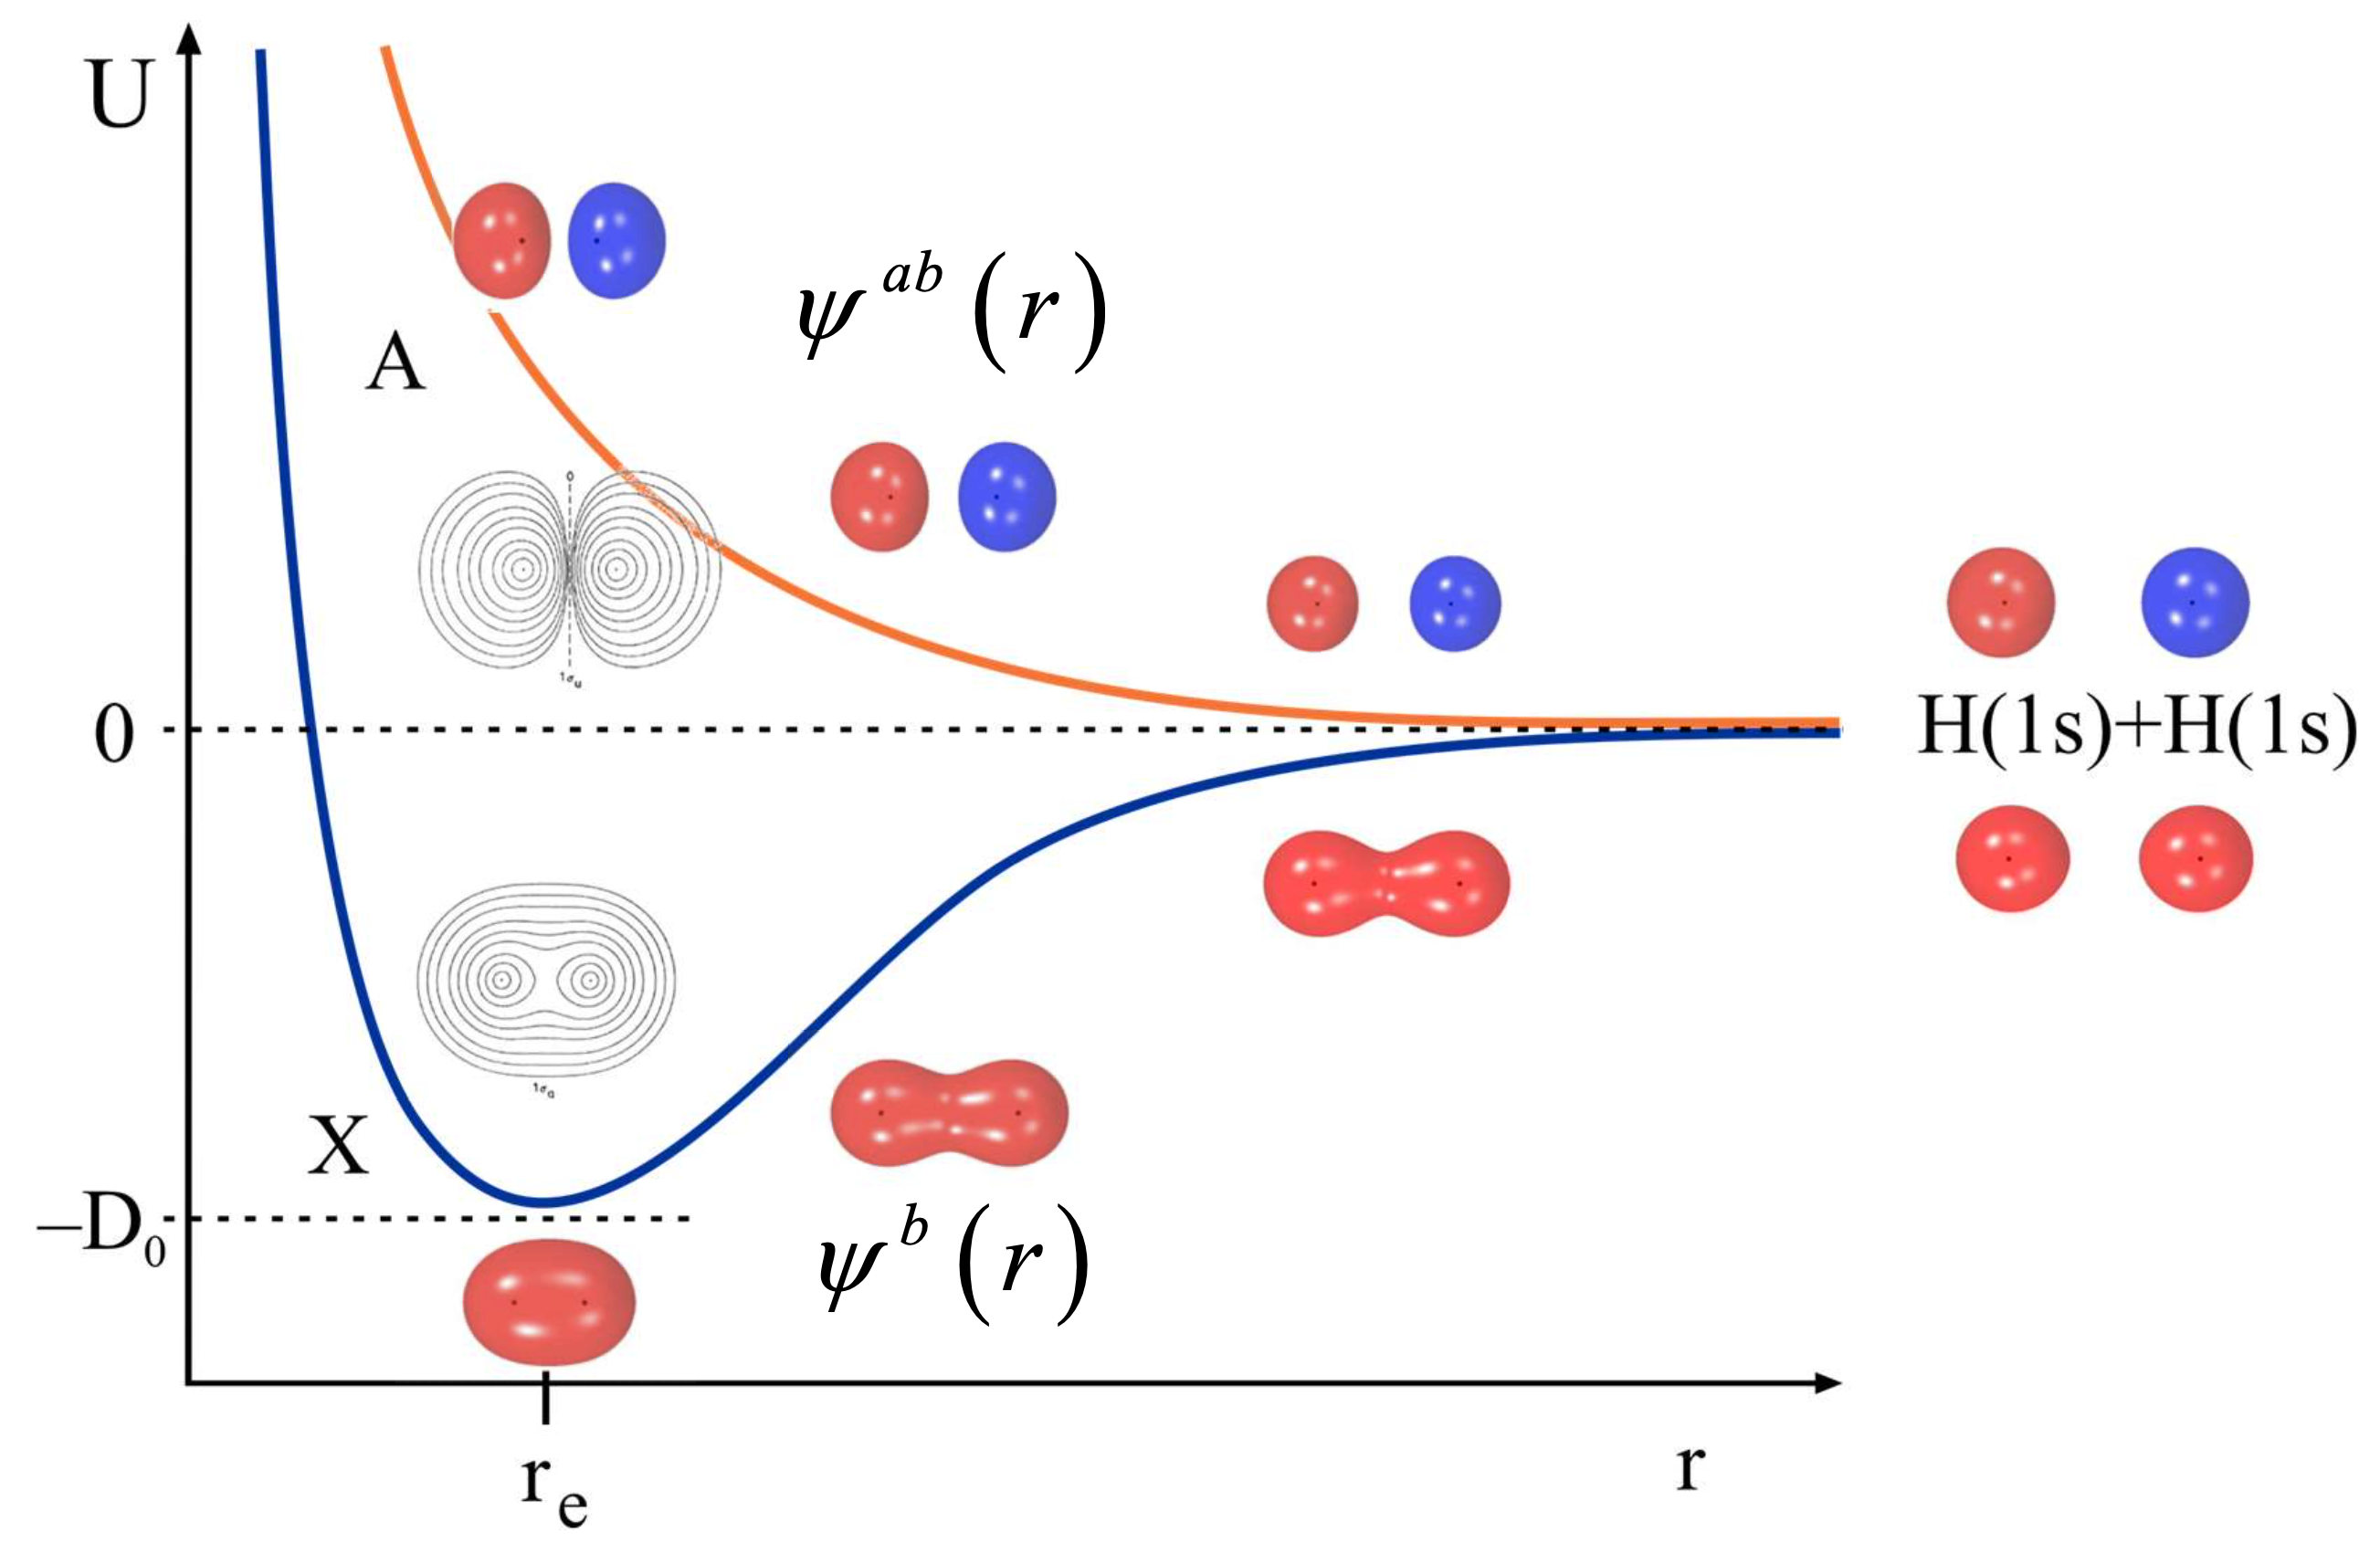
\includegraphics[width=0.5\linewidth]{BOH2.png}
        \caption{Born-Oppenheimer surfaces for \ce{H2}.}
        \label{fig:BOH2}
    \end{figure}
    \begin{itemize}
        \item Born-Oppenheimer surfaces characterize bonding.
        \begin{itemize}
            \item The curves/surfaces represent the possible ways in which electrons can interact and how the energy of the electrons in the system depends on the relative positions of the two hydrogen atoms.
        \end{itemize}
        \item The bonding and antibonding behavior of electrons originates from their quantum wavefunction nature since these wavefunctions can constructively and destructively interfere.
        \item With respect to \ce{H2}, the bonding and antibonding wavefunctions are, respectively,
        \begin{align*}
            \Psi^\text{b} &= c_1(r)\psi_{1s}^\text{H1}+c_2(r)\psi_{1s}^\text{H2}&
            \Psi^\text{ab} &= c_2(r)\psi_{1s}^\text{H1}-c_2(r)\psi_{1s}^\text{H2}
        \end{align*}
        \begin{itemize}
            \item Reason for the inversion of $c_2,c_1$ in the second line??
        \end{itemize}
        \item Conclusion: The BO approximation not only yields energies but also allows us to visualize the shape/electronic states of the molecule at different separations.
    \end{itemize}
    \item Electronic states.
    \begin{itemize}
        \item We can generalize the approach taken above to very complex systems.
        \item Examples include the MOs of \ce{H2O}, electron distribution of valence electrons in the HOMO and LUMO of chlorophyll a (one of the most important light-absorbing biological molecules) and caratenoids (other biological light-absorbing molecules), carbon nanotubes, and dyes.
        \item Wavefunctions describe the electron distribution in different states.
        \item The energy between the states is a lot! Circa $\SIrange{20000}{100000}{\per\centi\meter}=\SIrange[per-mode=symbol]{10}{50}{\kilo\joule\per\mole}$.
    \end{itemize}
    \item Having dealt with electronic states, how do we deal with nuclear ones?
    \item Nuclear degrees of freedom.
    \begin{figure}[H]
        \centering
        \begin{subfigure}[b]{0.3\linewidth}
            \centering
            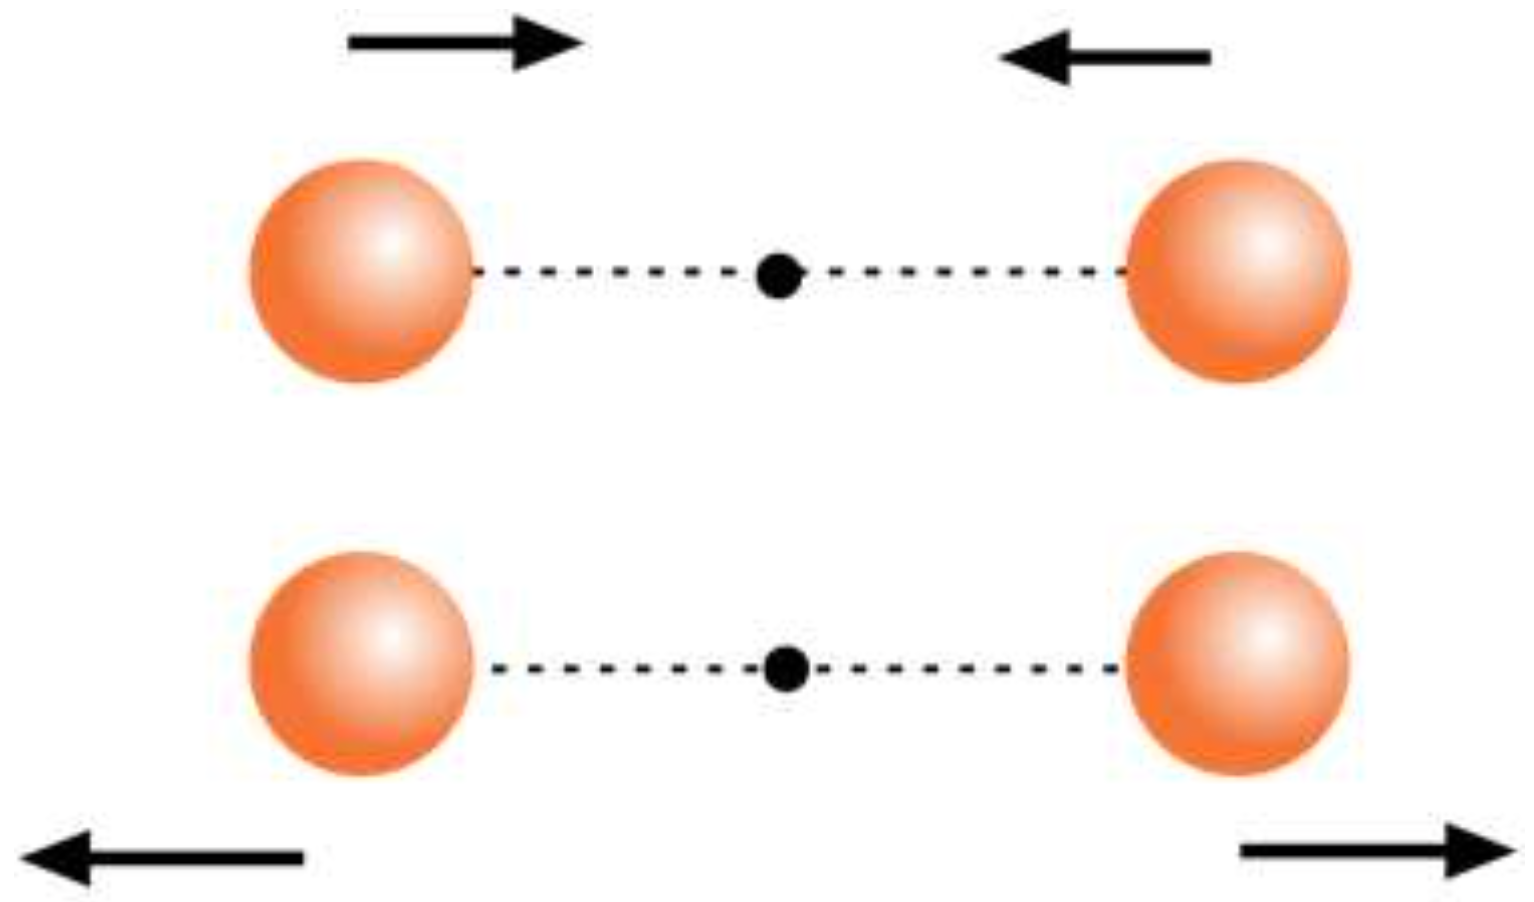
\includegraphics[width=0.8\linewidth]{nuclearMotiona.png}
            \caption{Vibration.}
            \label{fig:nuclearMotiona}
        \end{subfigure}
        \begin{subfigure}[b]{0.3\linewidth}
            \centering
            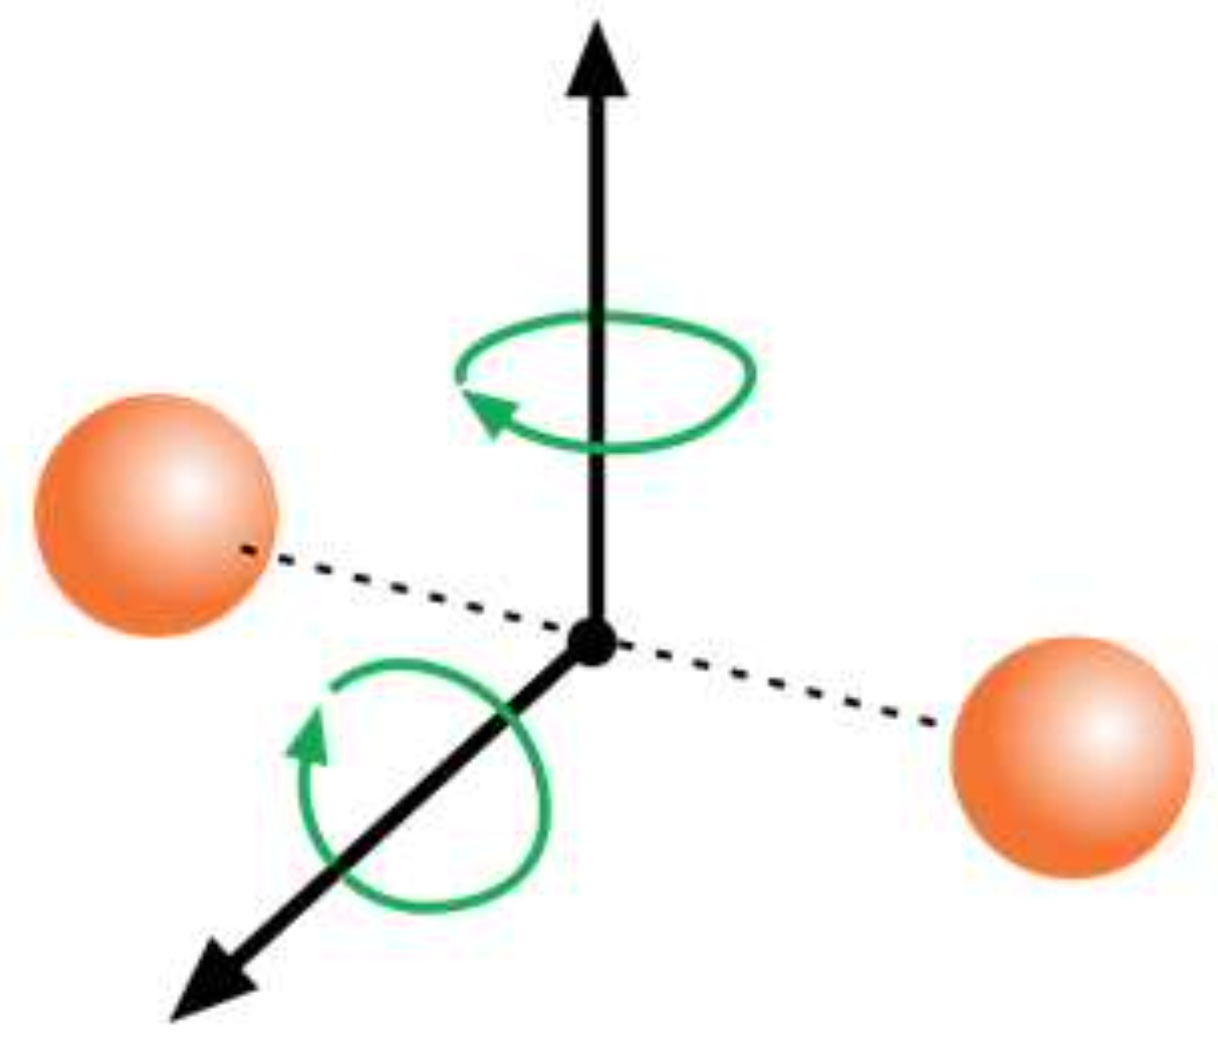
\includegraphics[width=0.63\linewidth]{nuclearMotionb.png}
            \caption{Rotation.}
            \label{fig:nuclearMotionb}
        \end{subfigure}
        \begin{subfigure}[b]{0.3\linewidth}
            \centering
            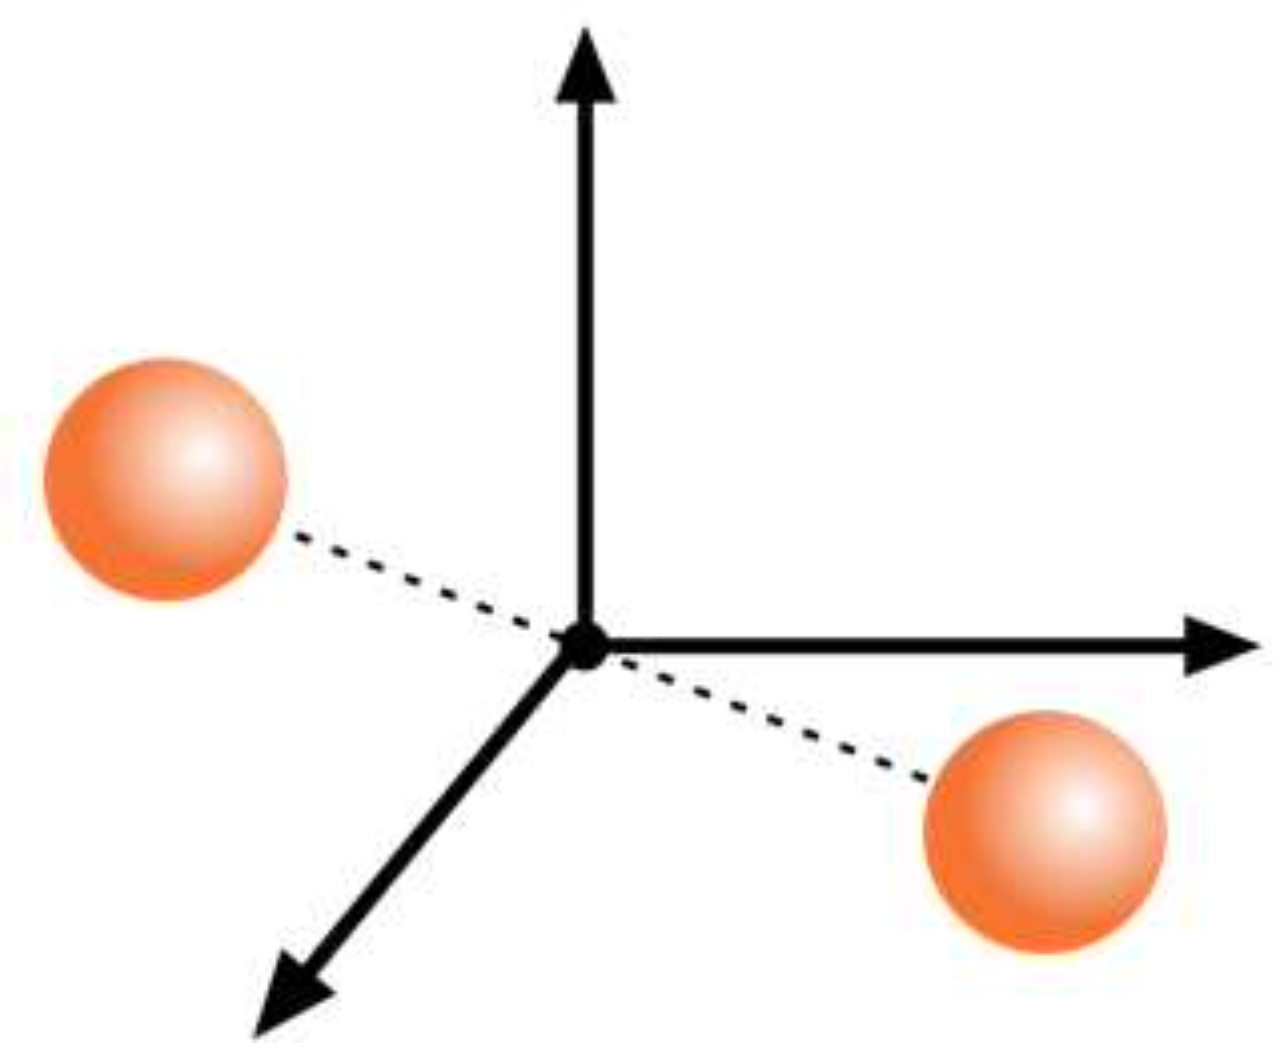
\includegraphics[width=0.63\linewidth]{nuclearMotionc.png}
            \caption{Translation.}
            \label{fig:nuclearMotionc}
        \end{subfigure}
        \caption{Modes of nuclear motion.}
        \label{fig:nuclearMotion}
    \end{figure}
    \begin{itemize}
        \item Three types with respect to the center of mass.
        \begin{enumerate}
            \item Vibration: Displacement of atoms relative to one another / COM fixed.
            \item Rotation: Motion about the COM.
            \item Translation: Motion of the COM.
        \end{enumerate}
        \item Translation is separated out during the transformation to internal coordinates.
        \item Vibration and rotation are separable independent motions.
        \begin{align*}
            E_\text{nuc} &= E_\text{vib}+E_\text{rot}&
            \Psi_\text{nuc} &= \Psi_\text{vib}\Psi_\text{rot}
        \end{align*}
        \begin{itemize}
            \item As we've discussed (see Figures \ref{fig:EMdipoleChange}-\ref{fig:EMrotationSync} and the associated discussion), these are the important ones for spectroscopy.
        \end{itemize}
    \end{itemize}
    \item Nuclear degrees of freedom in molecules.
    \begin{table}[h!]
        \centering
        \small
        \renewcommand{\arraystretch}{1.2}
        \begin{tabular}{c|cc}
                          & Linear & Nonlinear\\
            \hline
            Vibrational   & $3n-5$ & $3n-6$   \\
            Rotational    & 2      & 3        \\
            Translational & 3      & 3        \\
        \end{tabular}
        \caption{Nuclear DOFs in linear and nonlinear molecules.}
        \label{tab:linearNonDOF}
    \end{table}
    \begin{itemize}
        \item For a polyatomic molecule with $n$ atoms, there are $3n$ nuclear degrees of freedom.
        \item Linear and nonlinear molecules partition DOFs differently between vibration, rotation, and translation (see Table \ref{tab:linearNonDOF}).
        \item The vibrational DOFs exist as \textbf{normal modes}.
    \end{itemize}
    \item \textbf{Normal mode}: An independent vibration that doesn't move the COM.
    \begin{itemize}
        \item More on this later.
    \end{itemize}
    \pagebreak
    \item Vibrations.
    \begin{figure}[H]
        \centering
        \begin{subfigure}[b]{0.35\linewidth}
            \centering
            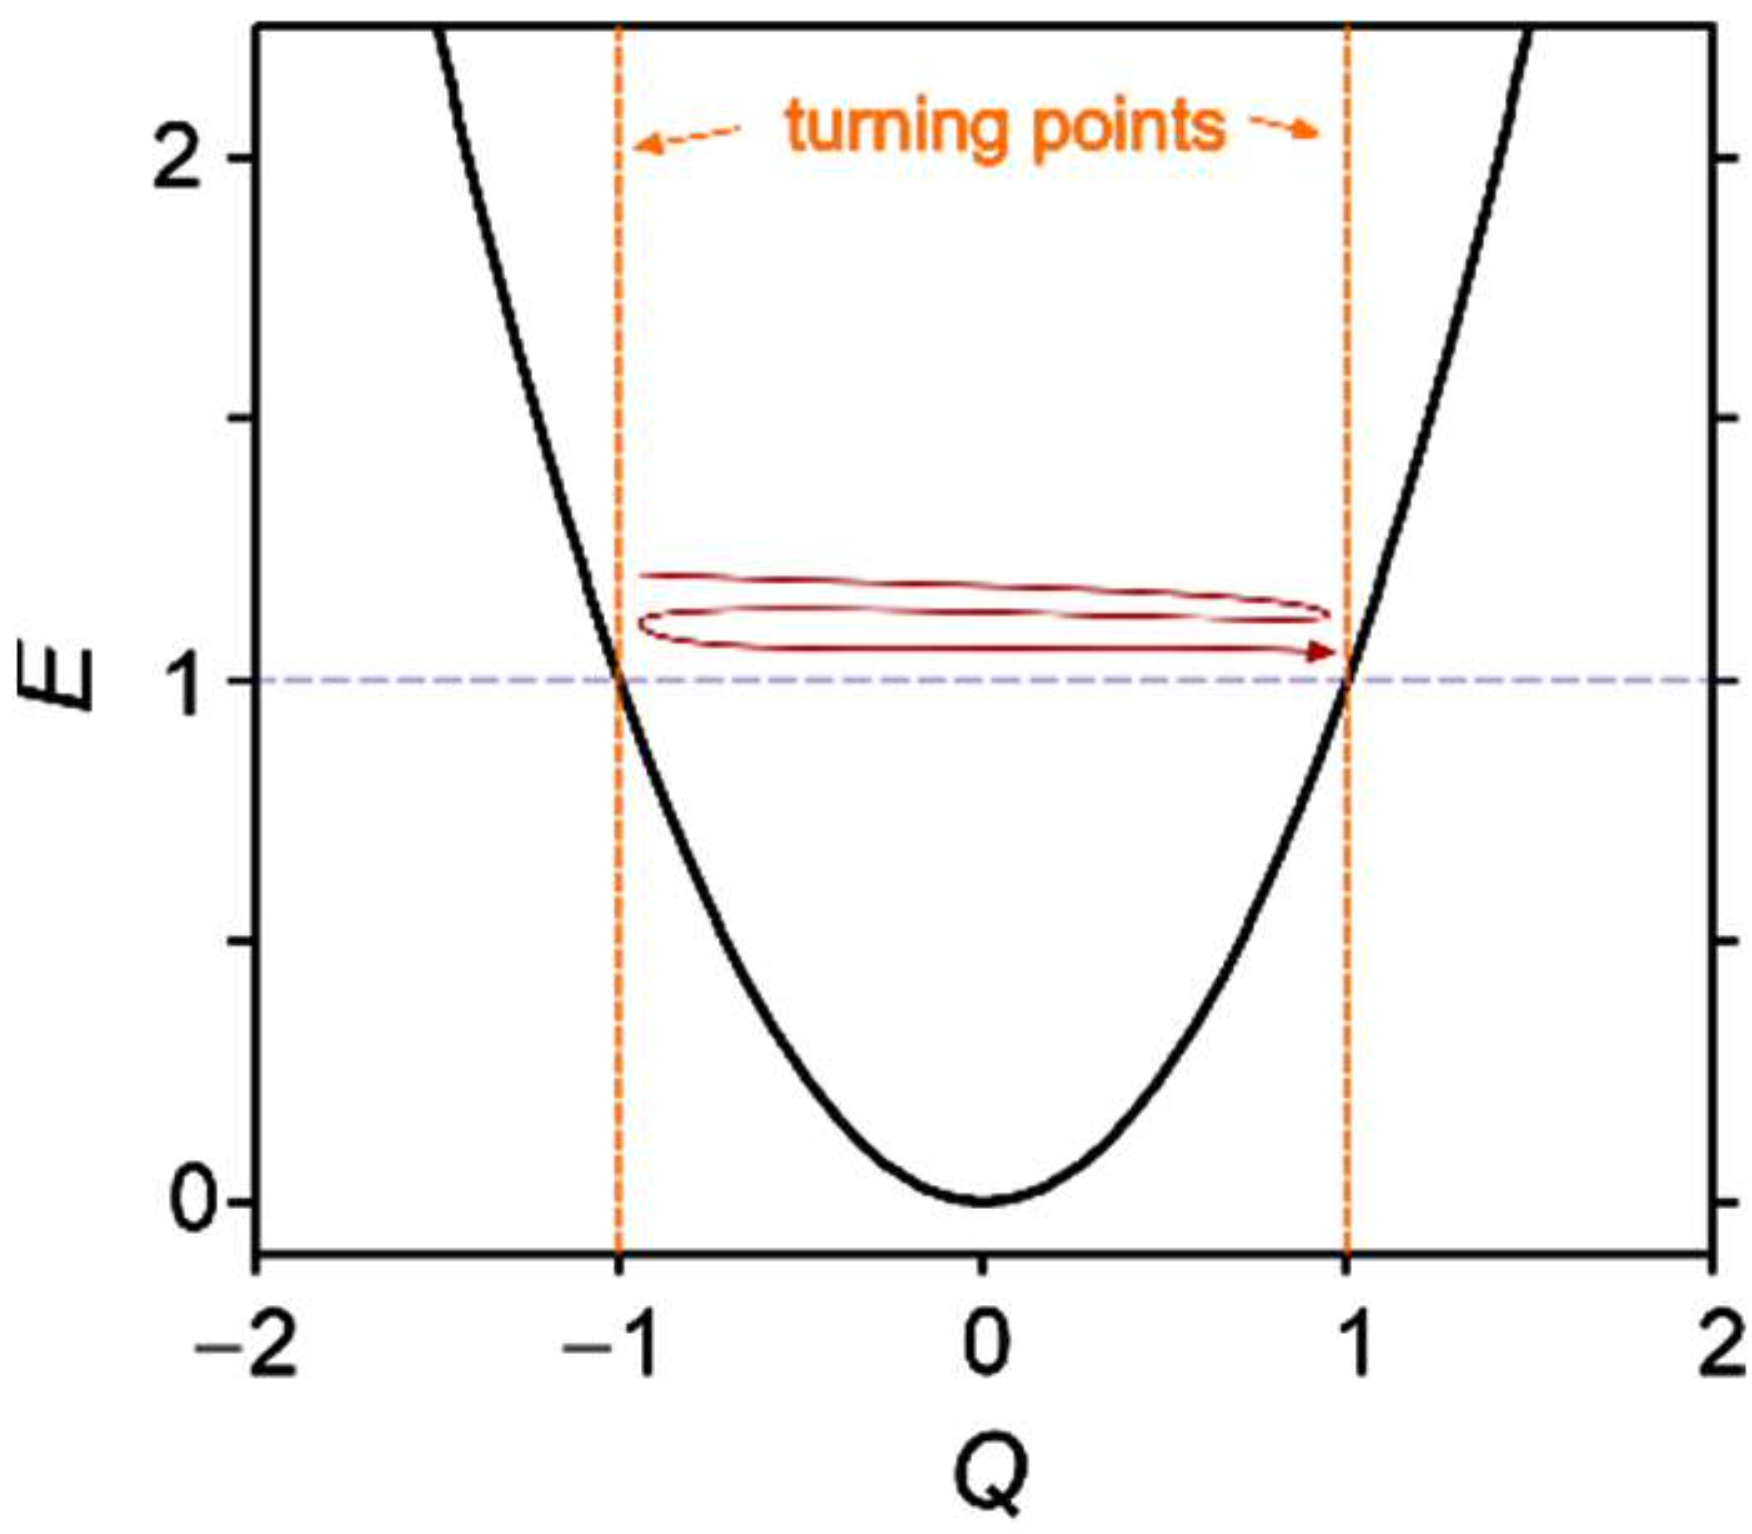
\includegraphics[width=0.8\linewidth]{vibrationalTreatmenta.png}
            \caption{Classical.}
            \label{fig:vibrationalTreatmenta}
        \end{subfigure}
        \begin{subfigure}[b]{0.35\linewidth}
            \centering
            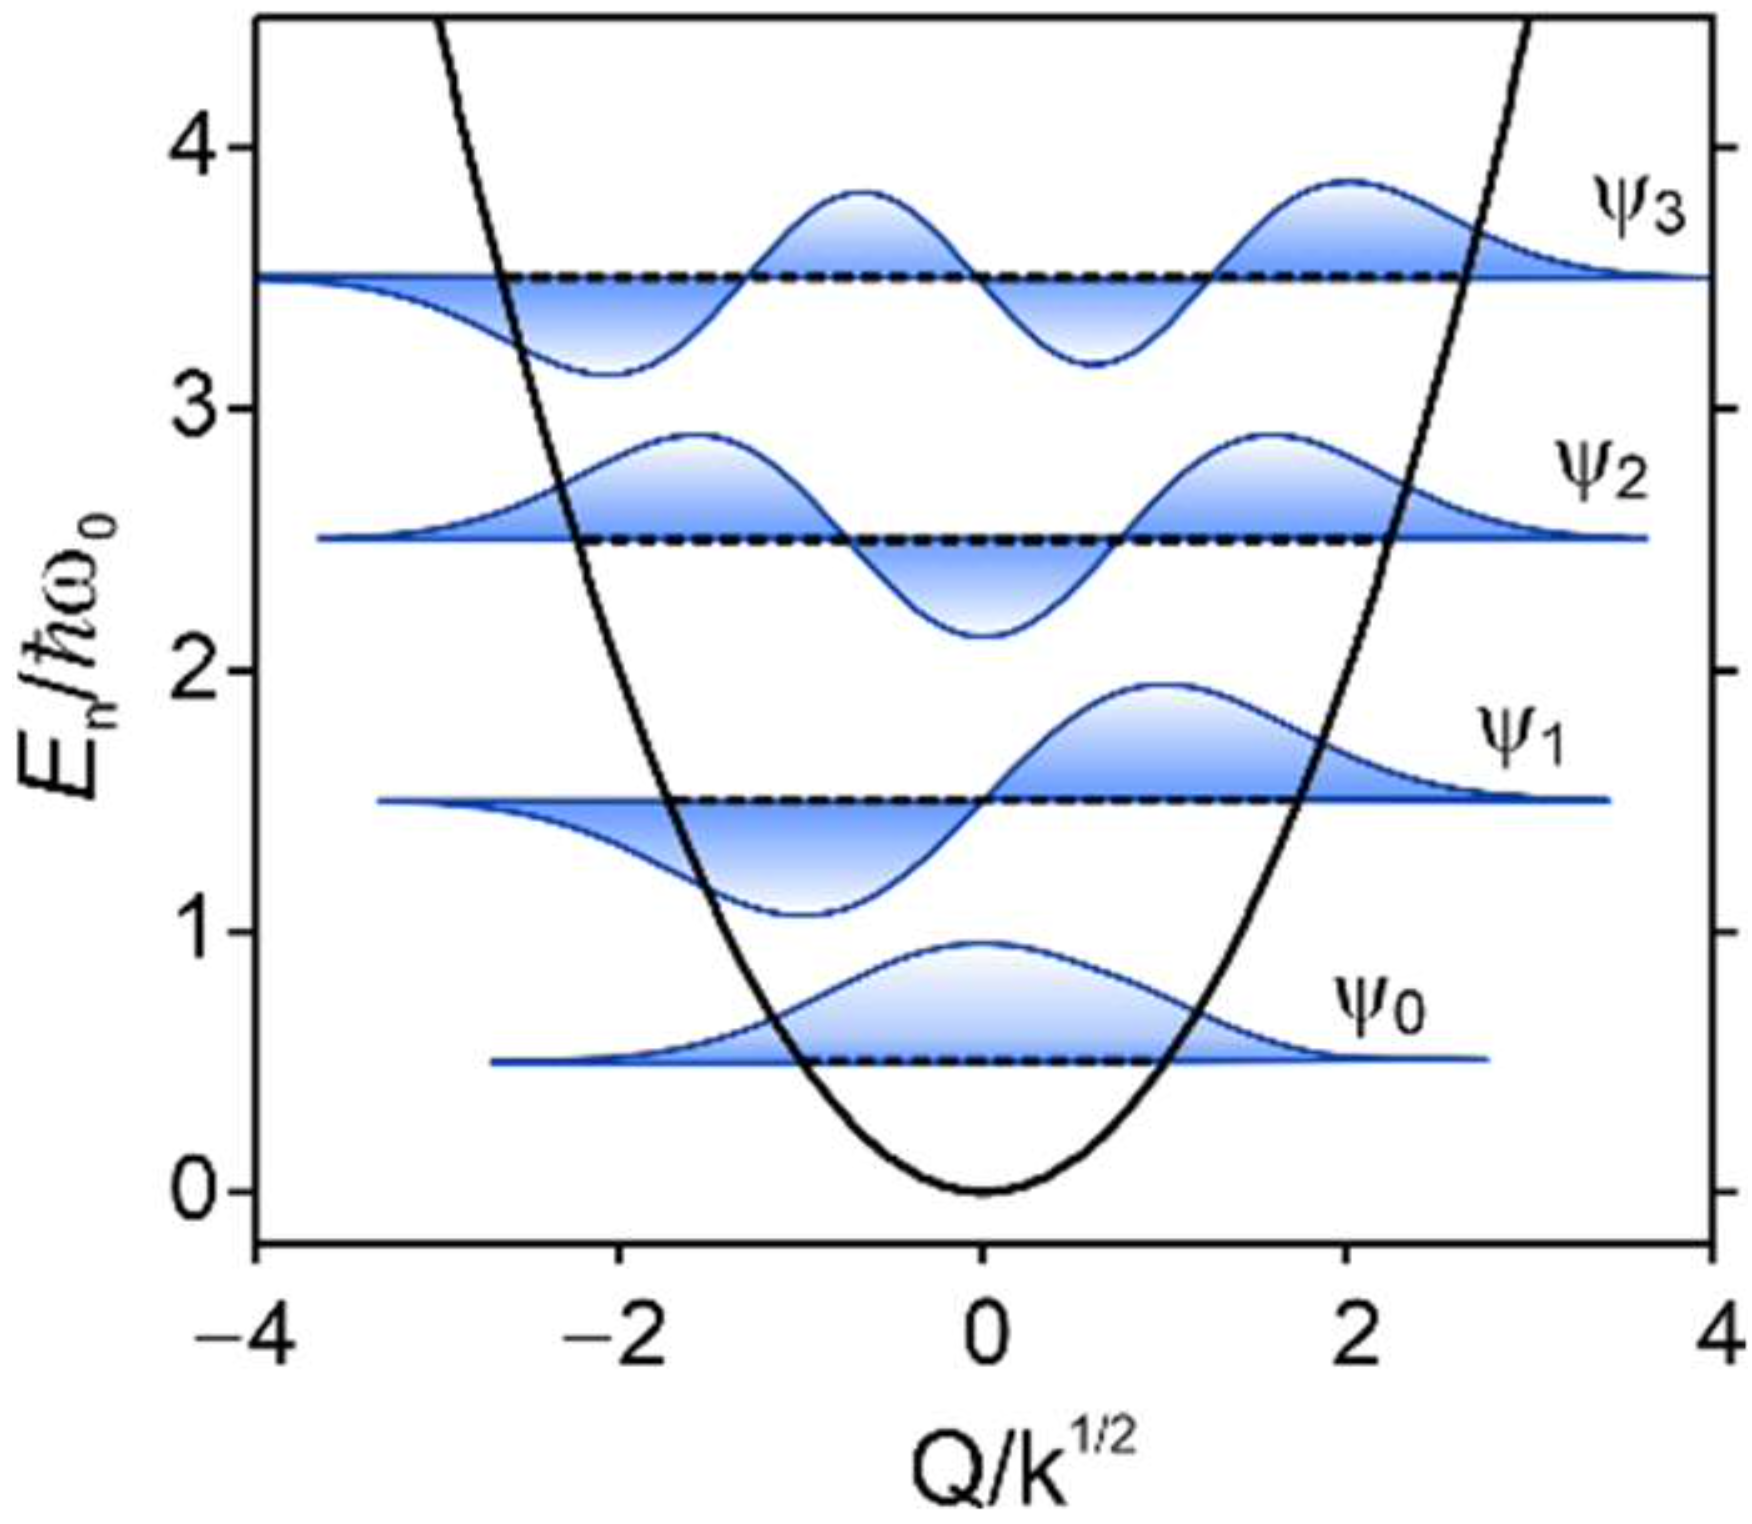
\includegraphics[width=0.8\linewidth]{vibrationalTreatmentb.png}
            \caption{Quantum.}
            \label{fig:vibrationalTreatmentb}
        \end{subfigure}
        \caption{Classical vs. quantum picture of vibration.}
        \label{fig:vibrationalTreatment}
    \end{figure}
    \begin{itemize}
        \item Classical treatment.
        \begin{itemize}
            \item We have a quadratic potential well.
            \item Any energy can be put into vibrational motion.
            \begin{itemize}
                \item More energy means a higher displacement.
            \end{itemize}
            \item Motion is periodic with classical turning points.
            \item Mathematically,
            \begin{align*}
                E &= V+T&
                    Q(t) &= A\sin\omega_0t\\
                &= \frac{1}{2}kQ^2+\frac{p^2}{2m}
            \end{align*}
        \end{itemize}
        \item Quantum treatment.
        \begin{itemize}
            \item Discrete energy levels corresponding to specific vibrational states.
            \item Vibrational wavefunctions $\psi_\text{vib}$ of $\chi_n$: Hermite polynomials.
        \end{itemize}
    \end{itemize}
    \item Quantum harmonic oscillator.
    \begin{itemize}
        \item Vibrational energy levels are given by
        \begin{equation*}
            E_\text{vib} = E_\nu
            = h\nu_e\left( v+\frac{1}{2} \right)
        \end{equation*}
        where $\nu_e$ can alternatively be expressed in either of the following forms.
        \begin{align*}
            \nu_e &= c\bar{\nu}_e&
            \nu_e &= \frac{1}{2\pi}\sqrt{\frac{k}{m_R}}
        \end{align*}
        \begin{itemize}
            \item The right form relates energy (via $\nu_e$) to the force constant of the harmonic oscillator.
        \end{itemize}
        \item Variable definitions.
        \begin{itemize}
            \item $\nu_e$ is the vibrational frequency.
            \item $v=0,1,2,\dots$ is the vibrational quantum number.
        \end{itemize}
        \item Typically, $\bar{\nu}_e\approx\SIrange{300}{3000}{\per\centi\meter}$.
        \item $h\nu_e$ is our unit of energy (the \textbf{quantum} of energy), and $E_0=h\nu_e/2$ is the zero-point energy.
        \begin{itemize}
            \item Recall that $E_0$ is derived by plugging $v=0$ into the $E_\text{vib}$ equation.
        \end{itemize}
        \item The spacing between adjacent vibrational levels is uniform and given by
        \begin{equation*}
            \Delta E = E_\nu-E_{\nu-1}
            = h\nu_e
        \end{equation*}
    \end{itemize}
    \item Rotation.
    \begin{figure}[H]
        \centering
        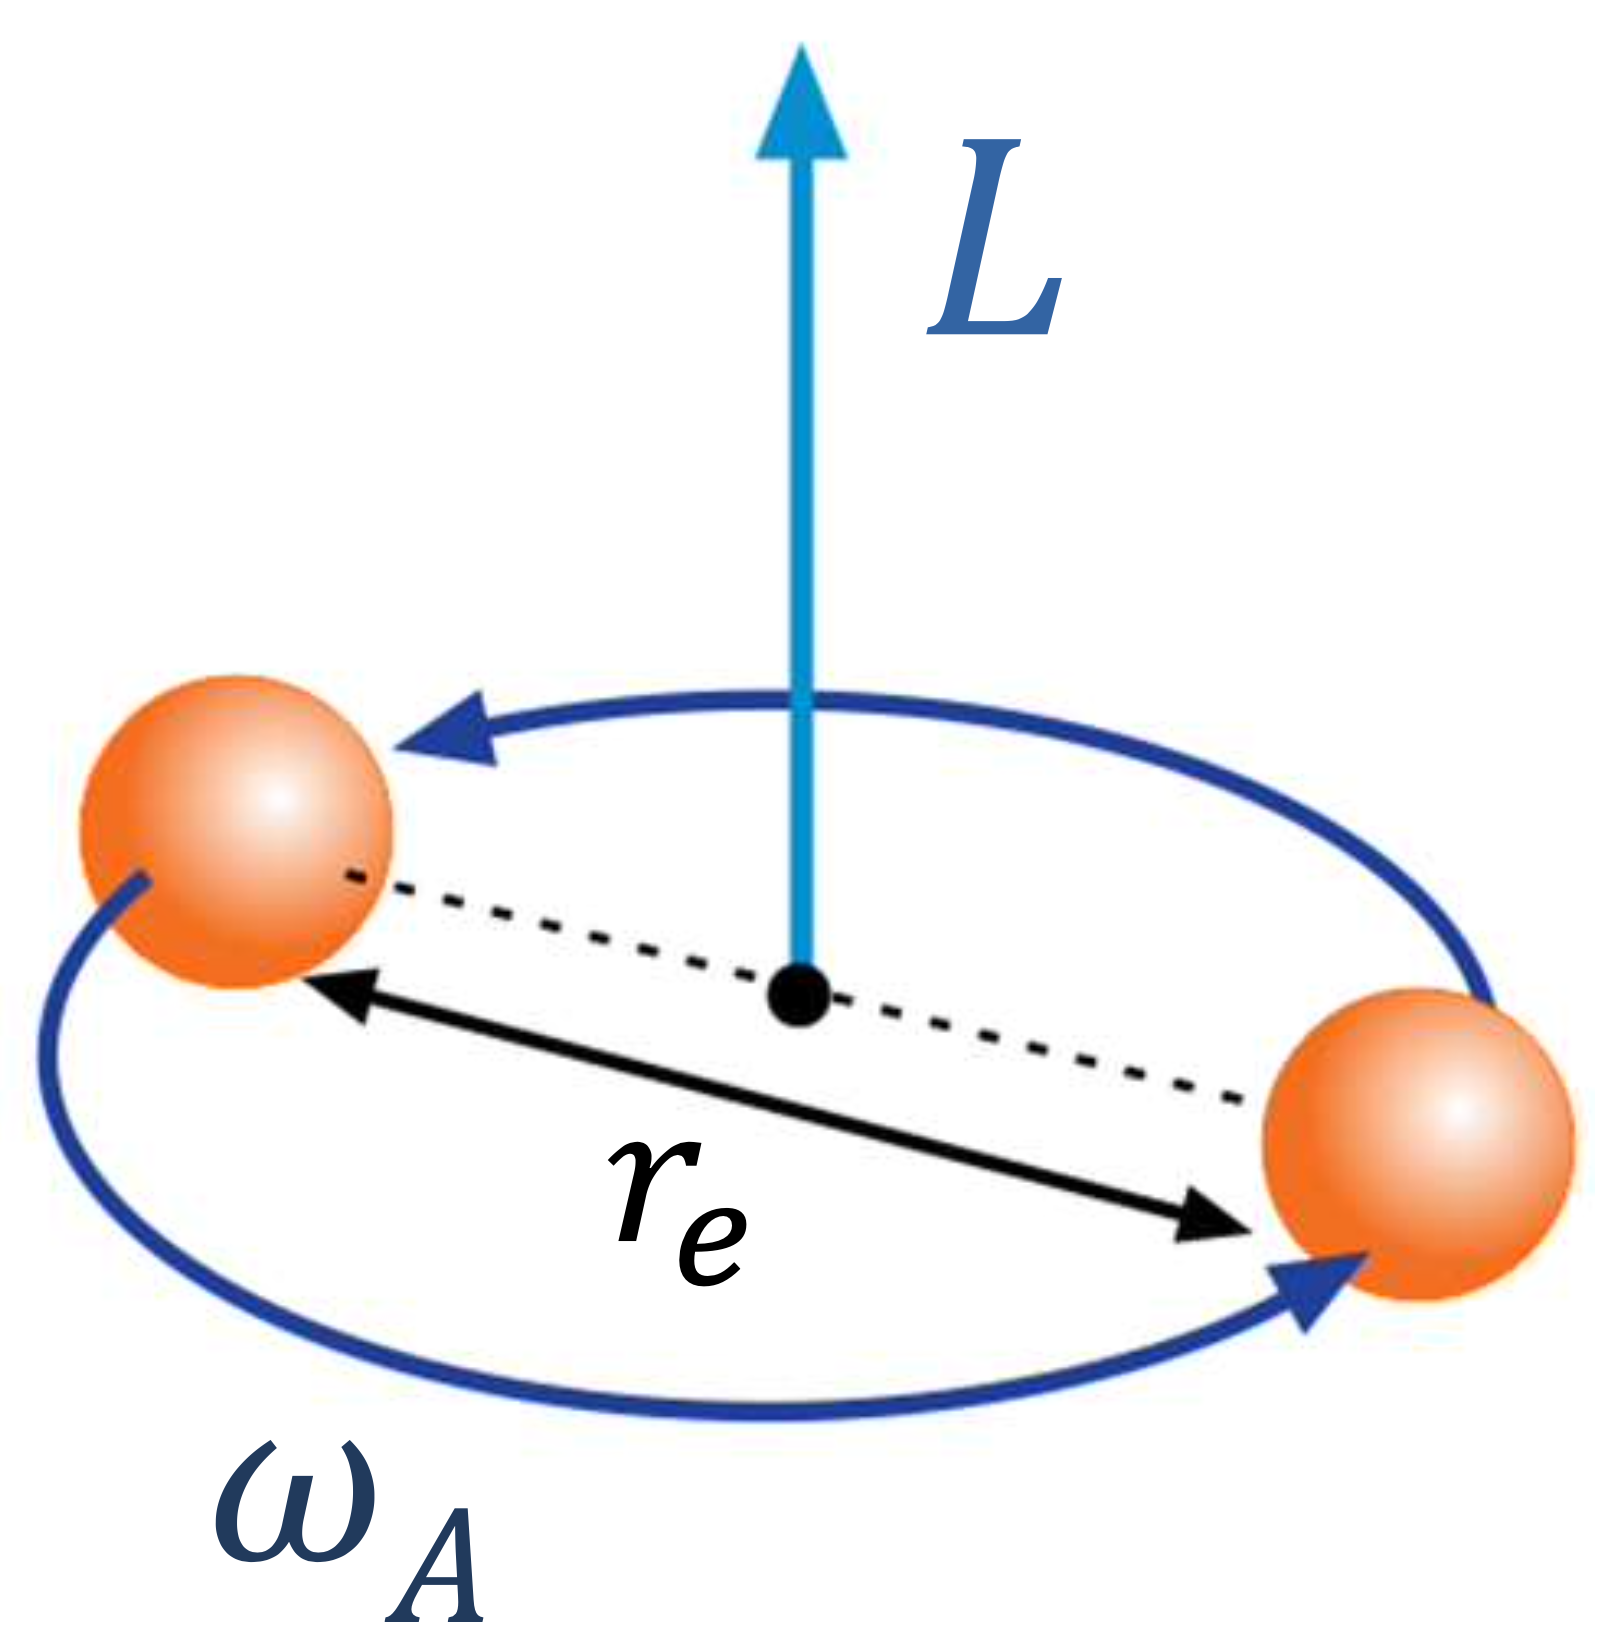
\includegraphics[width=0.16\linewidth]{rotationClassical.png}
        \caption{Classical rotation.}
        \label{fig:rotationClassical}
    \end{figure}
    \begin{itemize}
        \item Classically, rotation of a free object is governed by its angular momentum $L$, where
        \begin{equation*}
            L = I\omega_A
        \end{equation*}
        \item For a classical diatomic molecule\dots
        \begin{itemize}
            \item The moment of inertia is $I=m_Rr_e^2$;
            \item The energy of free rotation is purely kinetic, given by $E_\text{rot}=\frac{1}{2}I\omega_A^2=L^2/2I$.
        \end{itemize}
        \item Quantum mechanically, these expressions still hold. However, rotational angular momentum $L$ is quantized.
    \end{itemize}
    \item \textbf{Quantum rigid rotor}: Rotation occurs without any vibration or other configurational change with respect to the internal coordinates.
    \begin{figure}[h!]
        \centering
        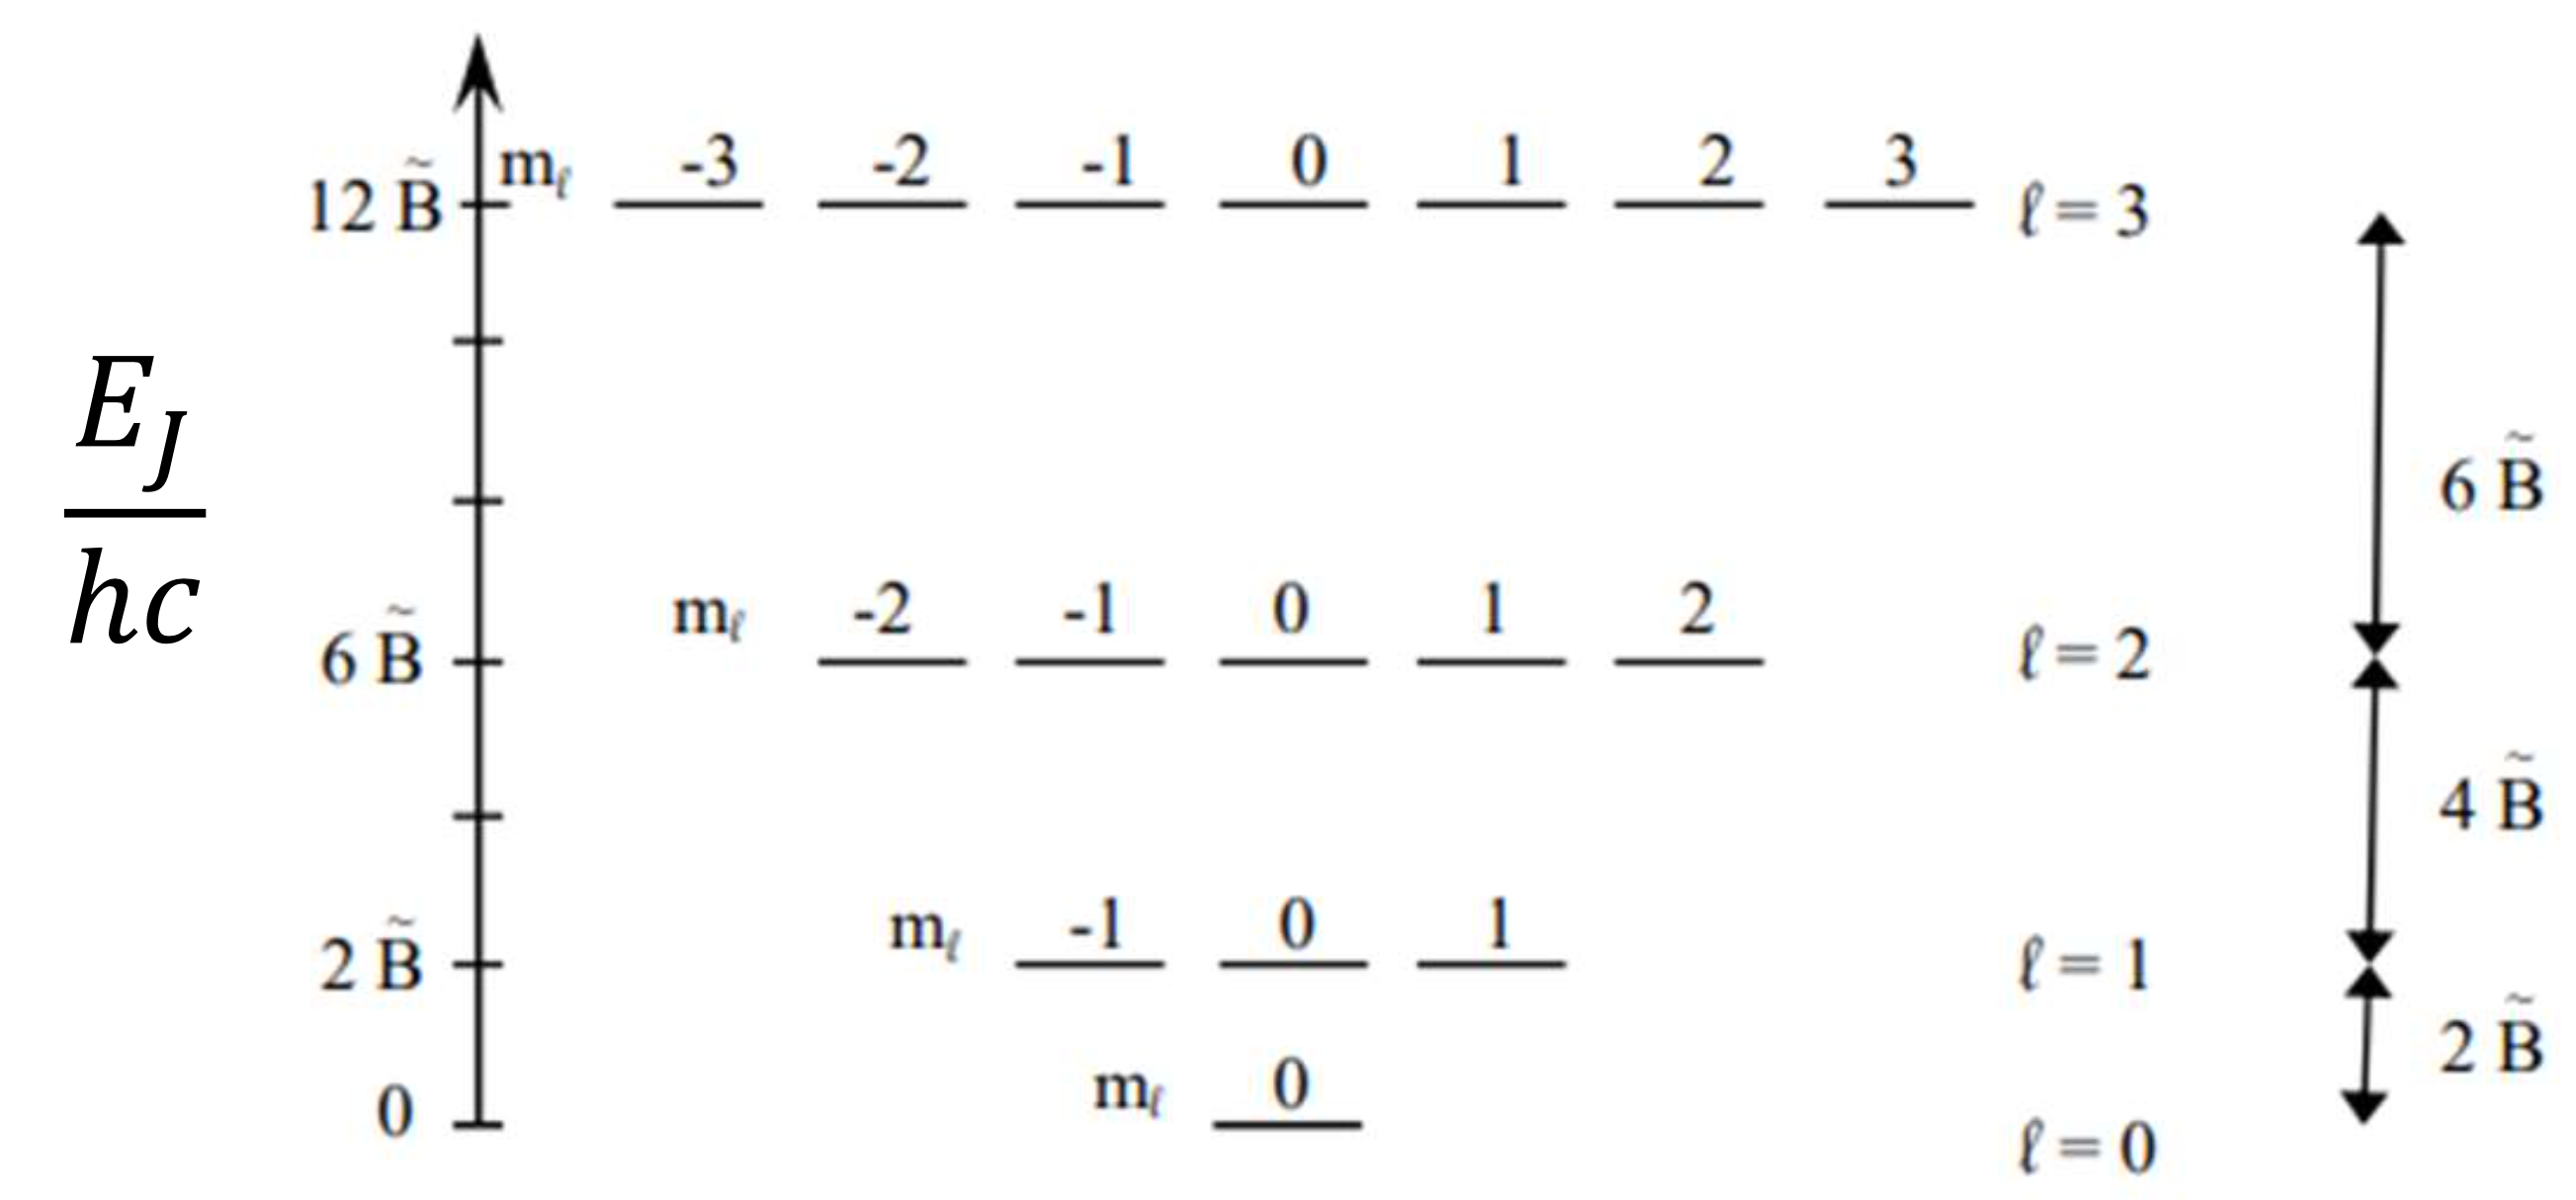
\includegraphics[width=0.6\linewidth]{rotationQuantum.png}
        \caption{Quantum rotation.}
        \label{fig:rotationQuantum}
    \end{figure}
    \begin{itemize}
        \item Rotational energy levels are given by
        \begin{equation*}
            E_\text{rot} = \frac{L^2}{2I}
            = \frac{\hbar^2}{2I}J(J+1)
            = hc\bar{B}J(J+1)
        \end{equation*}
        \item Variable definitions.
        \begin{itemize}
            \item $J=0,1,2,\dots$ is the rotational angular momentum quantum number.
            \item $\bar{B}=h/8\pi^2 cI$ is the rotational constant, which typically has value between \SIrange{0.1}{10}{\per\centi\meter}.
        \end{itemize}
        \item As $J$ increases, more and more rotational energy levels become available (see Figure \ref{fig:rotationQuantum}).
        \begin{itemize}
            \item Precisely, the degeneracy $g(J)$ of the $J^\text{th}$ rotational energy level is $g(J)=2J+1$.
            \item Degenerate energy levels are indexed by the azimuthal quantum number $M_J=0,\dots,\pm J$, which has to do with the projection of the angular momentum onto the axis of rotation.
        \end{itemize}
        \item The spacing between adjacent rotational energy levels is \emph{not} uniform (see Figure \ref{fig:rotationQuantum}).
        \begin{itemize}
            \item The spacing between the $M_J$ levels is uniform.
        \end{itemize}
    \end{itemize}
    \item Quantum mechanical energies.
    \begin{figure}[H]
        \centering
        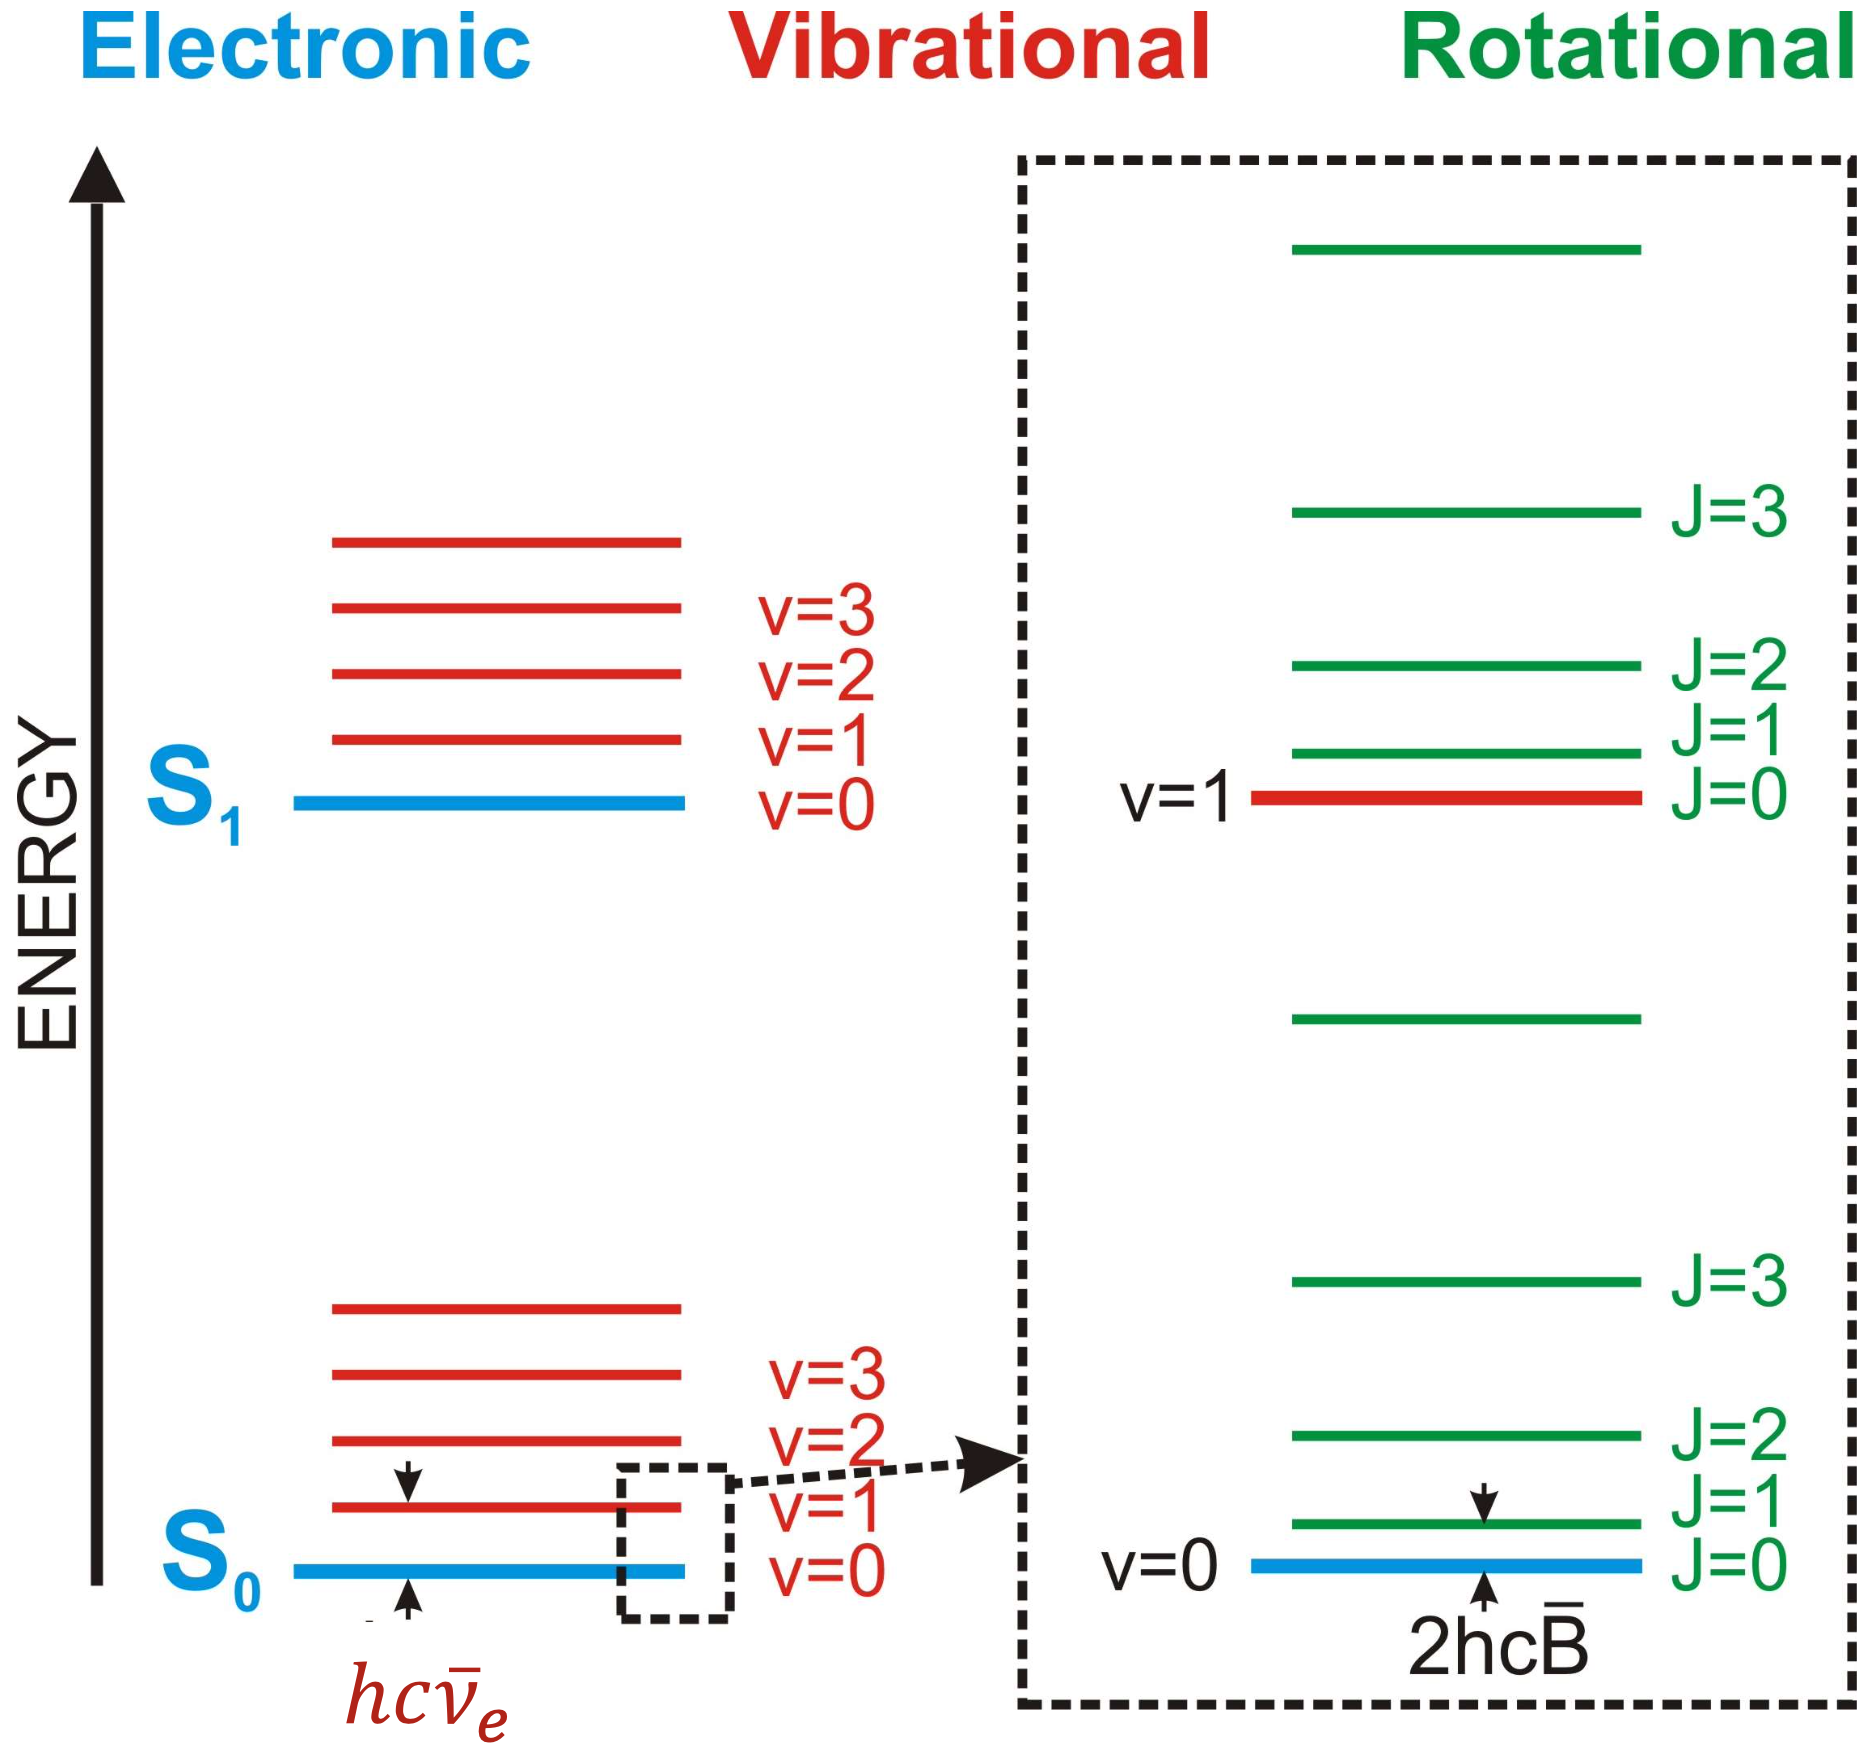
\includegraphics[width=0.4\linewidth]{qmechEnergySpacing.png}
        \caption{Electronic, vibrational, and rotational energy level spacing.}
        \label{fig:qmechEnergySpacing}
    \end{figure}
    \begin{itemize}
        \item Given the way that we approached the problem, we have that
        \begin{align*}
            E_\text{tot} &= E_\text{elec}+E_\text{vib}+E_\text{rot}+\cdots\\
            &= E_\text{elec}+hc\bar{\nu}_e\left( v+\frac{1}{2} \right)+hc\bar{B}J(J+1)+\cdots
        \end{align*}
        \begin{itemize}
            \item The energy can only take on discrete values (see Figure \ref{fig:qmechEnergySpacing}).
        \end{itemize}
        \item Note that the typical energy range for\dots
        \begin{itemize}
            \item $E_\text{elec}$ is \SIrange{e4}{e5}{\per\centi\meter};
            \item $E_\text{vib}$ is \SIrange{e2}{e3}{\per\centi\meter};
            \item $E_\text{rot}$ is \SIrange{e-1}{e1}{\per\centi\meter}.
            \item The scale of electronic differences, vs. vibrational differences, vs. rotational differences is shown in Figure \ref{fig:qmechEnergySpacing}.
        \end{itemize}
        \item We can summarize the state of the system from an energy point of view by specifying vibrational and rotational constants ($\bar{\nu}_e$ and $\bar{B}$) and their associated quantum numbers ($\nu$ and $J$).
    \end{itemize}
    \item Wrap up.
    \begin{itemize}
        \item We have taken step one toward a quantum description of spectroscopy.
        \begin{itemize}
            \item Today: The wavefunction and energy of quantum states.
            \item Next time: Add light into the mix.
        \end{itemize}
        \item Separation of electronic, vibrational, and rotational motion in molecules leads to independent contributions to the energy via
        \begin{align*}
            E_\text{tot} &= E_\text{elec}+E_\text{vib}+E_\text{rot}&
            \Psi &= \Psi_\text{elec}\Psi_\text{vib}\Psi_\text{rot}
        \end{align*}
        \item For spectroscopy, we can specify the state of a molecule with $E_\text{elec}$ relative to the ground electronic state, the vibrational and rotational constants $\bar{\nu}_e$ and $\bar{B}_e$, and associated quantum numbers.
    \end{itemize}
\end{itemize}



\section{Lab 1: UV-VIS}
\subsection*{Ocean Optics Procedure}
\begin{itemize}
    \item This is the solution-phase experiment.
    \item See document for experimental procedure. No theory here (see Rowan's slides for that).
    \item This experiment allows us to calculate the extinction coefficient of iodine.
\end{itemize}


\subsection*{Lab Manual}
\begin{itemize}
    \item This is the gas-phase experiment.
    \item \textbf{X state}: The ground electronic state.
    \item \textbf{B state}: An excited electronic state.
    \item Purpose of the experiment: Take a \SIrange{500}{600}{\nano\meter} UV/Vis absorption spectrum of gaseous \ce{I2}, and use it to calculate several spectroscopic constants.
    \item Introduction to the theory.
    \begin{itemize}
        \item Refer to Chapter 13 of \textcite{bib:McQuarrieSimon} for additional context on the following.
    \end{itemize}
    \item The energy of a spectroscopic transition (in \si{\per\centi\meter}) is given by
    \begin{equation*}
        \omega(v',v'',J',J'') = T_e'-T_e''+G'(v')-G''(v'')+F'(J')-F''(J'')
    \end{equation*}
    \item Variable definitions (all quantities in \si{\per\centi\meter}).
    \begin{itemize}
        \item $T_e$ is the electronic energy.
        \item $G(v)$ is the energy of the vibrational energy level with vibrational quantum number $v$.
        \item $F(J)$ is the energy of the rotational energy level with rotational quantum number $J$.
        \item Single primes refer to the upper state (in this case, the B state) and double primes refer to the lower state (in this case, the X state).
    \end{itemize}
    \item We set the zero of energy by defining
    \begin{equation*}
        T_e'' = 0
    \end{equation*}
    \item To account for anharmonicity, vibrational energy levels can be written as a power series expansion in $(v+1/2)$.
    \begin{equation*}
        G(v) = \omega_e(v+1/2)-\omega_ex_e(v+1/2)^2+\omega_ey_e(v+1/2)^3+\cdots
    \end{equation*}
    \begin{itemize}
        \item In the above equation, $\omega_e=\omega$ is the energy of the transition in wavenumbers, and $x_e,y_e,\dots$ are anharmonicity constants.
    \end{itemize}
    \item Similarly, rotational energy levels can be written in a power series expansion in $(J(J+1))$.
    \begin{equation*}
        F_v(J) = B_vJ(J+1)+D_vJ^2(J+1)^2+\cdots
    \end{equation*}
    \item In both the vibrational and rotational expansion, we only retain enough terms to adequately fit the spectroscopic data.
    \item Under our experimental conditions\dots
    \begin{itemize}
        \item Resolution will not be good enough to resolve rotational structure. Additionally, the cubic term of $G(v)$ can be neglected. Thus, \emph{our} form of the transition energy is
        \begin{align*}
            \omega(v',v'') &= \omega_\text{el}+G'(v')-G''(v'')\\
            &= \omega_\text{el}+\omega_e'(v'+1/2)-\omega_e'x_e'(v'+1/2)^2-\omega_e''(v''+1/2)+\omega_e''x_e''(v''+1/2)^2
        \end{align*}
        where $\omega_\text{el}=T_e'-T_e''$.
        \item $v,J$ in $(v',J'),(v'',J'')$ can take on any integer value in theory, but in practice, only a few show up.
        \begin{itemize}
            \item Indeed, the most intense transitions will be from level $v''=0$ and they will decrease in intensity as $v''$ increases.
            \item Additionally, there will be transitions to several values of $v'$. No \emph{simple} rules govern the intensities.
        \end{itemize}
        \item Also expect to see some overlap.
    \end{itemize}
    \item Several references are listed. These describe how to analyze the spectra in more detail.
    \item The experimental setup and procedure is described.
    \item We now move into data analysis.
    \item We analyze the spacing between electrovibrational transitions to determine the shape of the potential energy surfaces of the X and B states of \ce{I2}.
    \begin{itemize}
        \item In other words, any absorption peak we observe in our recorded spectrum corresponds to promotion of an electron from some vibrational energy level $v''=0,1,2$ in the ground electronic (X) state to some vibrational energy level $v'=0,1,2,\dots$ in the first excited (B) state. The spacing between these peaks allows us to calculate the necessary anharmonicity constants. We can then plug these back into a Morse potential.
    \end{itemize}
    \item The following well-established reference points will allow us to label all peaks in our spectrum.
    \begin{table}[h!]
        \centering
        \small
        \renewcommand{\arraystretch}{1.2}
        \begin{tabular}{|c|c|c|c|c|c|c|c|c|c|}
            \hline
            $\lambda$ (\si{\nano\meter}) & 541.2 & 539.0 & 536.9 & 571.6 & 568.6 & 565.6 & 595.7 & 592.0 & 588.5\\
            \hline
            $\nu'$ & 27 & 28 & 29 & 18 & 19 & 20 & 13 & 14 & 15\\
            \hline
            $\nu''$ & 0 & 0 & 0 & 1 & 1 & 1 & 2 & 2 & 2\\
            \hline
        \end{tabular}
        \caption{Established reference points in the UV/Vis spectrum of \ce{I2}.}
        \label{tab:UVVisI2References}
    \end{table}
    \item As per the above, we can calculate that
    \begin{align*}
        \Delta\omega(v') ={}& \omega(v'+1,v'')-\omega(v',v'')\\
        \begin{split}
            ={}& \omega_\text{el}+\omega_e'(v'+3/2)-\omega_e'x_e'(v'+3/2)^2-\omega_e''(v''+1/2)+\omega_e''x_e''(v''+1/2)^2\\
            &-\left[ \omega_\text{el}+\omega_e'(v'+1/2)-\omega_e'x_e'(v'+1/2)^2-\omega_e''(v''+1/2)+\omega_e''x_e''(v''+1/2)^2 \right]
        \end{split}\\
        \begin{split}
            ={}& \omega_e'(3/2)-\omega_e'x_e'\left( {v'}^2+3v'+9/4 \right)\\
            &-\left[ \omega_e'(1/2)-\omega_e'x_e'\left( {v'}^2+v'+1/4 \right) \right]
        \end{split}\\
        ={}& \omega_e'-2\omega_e'x_e'(v'+1)
    \end{align*}
    \begin{itemize}
        \item Thus, a \textbf{Birge-Sponer plot} can be used to calculate $\omega_e'$ and $x_e'$.
    \end{itemize}
    \item \textbf{Birge-Sponer plot}: A linear plot of $\Delta\omega(v)$ vs. $v+1$.
    \begin{itemize}
        \item As per the above, the line of best fit should have slope $-2\omega_ex_e$ and $y$-intercept $\omega_e$.
    \end{itemize}
    \item Similarly,
    \begin{equation*}
        \Delta\omega(v'') = \omega(v',v''+1)-\omega(v',v'')
        = \omega_e''-2\omega_e''x_e''(v''+1)
    \end{equation*}
    \begin{itemize}
        \item Once again, a Birge-Sponer plot enables the calculation of $\omega_e''$ and $x_e''$.
    \end{itemize}
    \item Relating $\omega_e',\omega_e'',x_e',x_e''$ to the Morse potential for the X and B states.
    \begin{itemize}
        \item Consider the general Morse potential function
        \begin{equation*}
            U(r) = D_e(\e[-\beta(r-r_e)]-1)^2
        \end{equation*}
        \item We will take it as God-given for now that
        \begin{align*}
            D_e &= \frac{\omega_e(1/x_e-x_e)}{4}&
            \beta &= \sqrt{\frac{k_e}{2hcD_e}}
        \end{align*}
        \begin{itemize}
            \item Recall that the force constant $k_e$ is equal to the curvature at the bottom of the well, i.e.,
            \begin{equation*}
                k_e = \left( \pdv[2]{U(r)}{r} \right)_{r_e}
                = \mu(2\pi c\omega_e)^2
            \end{equation*}
            where $\mu$ is the reduced mass of the system in question and $c$ is the speed of light in \si{\centi\meter\per\second}.
        \end{itemize}
    \end{itemize}
    \item Describing dissociation.
    \begin{itemize}
        \item Recall that dissociation occurs from the ground vibrational state $v''=0$, not the potential energy minimum at $U(r_e'')$.
        \item Thus, the dissociation energy $D_0$ is offset from $D_e$ by $G(0)$. In particular,
        \begin{equation*}
            D_0 = D_e-G(0)
            = \left[ \frac{\omega_e(1/x_e-x_e)}{4} \right]-\left[ \frac{\omega_e}{2}-\frac{\omega_ex_e}{4} \right]
            = \frac{\omega_e(1/x_e-2)}{4}
        \end{equation*}
    \end{itemize}
    \item Calculating the energy difference $T_e$ between the energy minima of the X and B states.
    \begin{itemize}
        \item We have that
        \begin{equation*}
            T_e = D_e''+E(\ce{I^*})-D_e'
        \end{equation*}
        where $E(\ce{I^*})$ is the energy of an excited iodine atom produced when the B state of \ce{I2} dissociates.
        \begin{itemize}
            \item Refer to Figure \ref{fig:UVVisI2Energy} to rationalize this expression.
            \item $E(\ce{I^*})\approx\SI{7603.15}{\per\centi\meter}$.
        \end{itemize}
    \end{itemize}
    \item A plot summarizing all quantities discussed thus far.
    \begin{figure}[H]
        \centering
        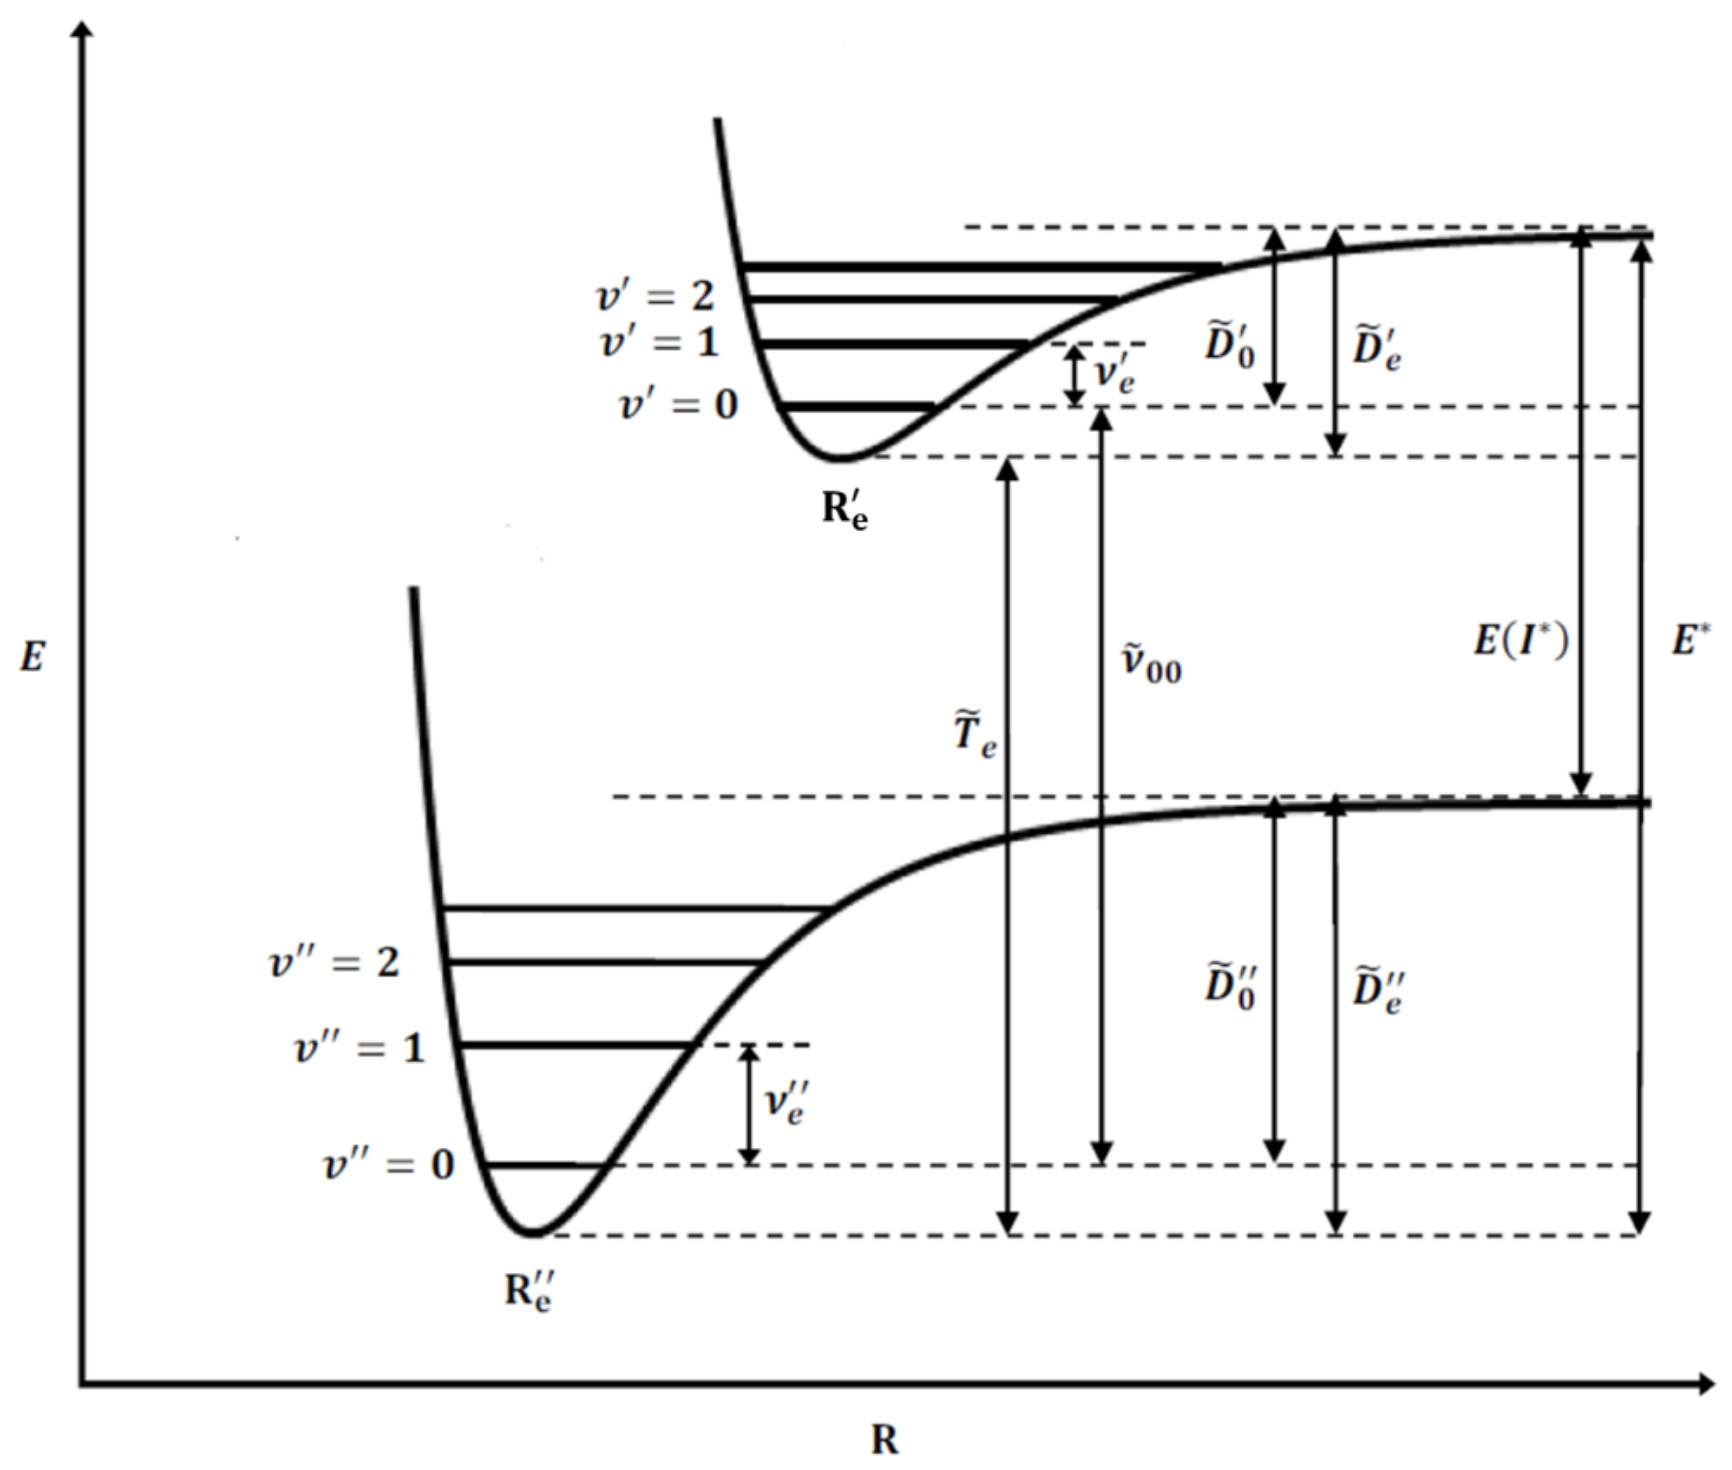
\includegraphics[width=0.7\linewidth]{UVVisI2Energy.png}
        \caption{The potential curves and spectroscopic quantities pertinent to \ce{I2}.}
        \label{fig:UVVisI2Energy}
    \end{figure}
    \item The document discusses an alternate way to analyze the data using parabolic least squares regression.
    \item The document includes instructions for the short lab report.
\end{itemize}


\subsection*{Rowan's Introduction to the UV-VIS Experiment}
\begin{itemize}
    \item Reviews the basics of absorption spectroscopy, today's experimental setups, and the expected analysis.
    \item Information on error propagation.
\end{itemize}


\subsection*{Quantities from the Experiment}
\begin{itemize}
    \item The original concentration of \ce{I2} in \ce{CHCl3} was \SI{0.01}{\molar} (\SI{0.1357}{\gram} in \SI{50}{\milli\liter}).
    \item We diluted \SI{0.7}{\milli\liter} of this solution to a volume of \SI{25}{\milli\liter}.
    \begin{itemize}
        \item This brought us into a region where Beer's law is linear.
    \end{itemize}
    \item The path length (width of the cuvette) is $b=\SI{1}{\centi\meter}$.
    \item \textbf{Beer's law}: The following relationship, where $A$ is peak absorbance, $\varepsilon$ is the extinction coefficient, $b$ is the path length, and $C$ is the concentration. \emph{Given by}
    \begin{equation*}
        A = \varepsilon bC
    \end{equation*}
\end{itemize}




\end{document}